\documentclass[11pt,a4paper]{ctexart}
\usepackage[margin=2.4cm]{geometry}
\usepackage{graphicx}
\usepackage{booktabs}
\usepackage{amsmath,amssymb}
\usepackage{array}
\usepackage[table]{xcolor}
\usepackage{natbib}
\usepackage{caption}
\captionsetup{font=small,labelfont=bf}
\usepackage[colorlinks=true,linkcolor=blue!60!black,citecolor=blue!60!black,urlcolor=blue!60!black]{hyperref}
\setlength{\parskip}{2pt}
\graphicspath{{../inputs/figures/}}

\title{基于因果匀速外推的单目交通视频短时预判：\\实现、误差分布刻画与系统性负结果}
\author{匿名作者}
\date{}

\begin{document}
\maketitle

\begin{abstract}
固定监控相机看得见当下，看不见下一步；而为存量机位换装雷达的成本不可承受。
本文交付一个纯视觉、因果的短时预判系统：输入 2$\sim$30 秒单目视频，输出带类型与
预判位置的连续视频，预判梯度为 0.1、0.5、1、2 秒。系统在单张 8\,GB 消费级显卡上
完成训练与推理，端到端 0.24\,s/帧。\textbf{结果}：目标域检测 mAP50 为 0.637，
规范口径下每帧可预判目标 14.87 个（占检出目标 44.6\%），1 秒预判中位误差 33.4
像素，轨迹跳变 18.3 次/千帧。\textbf{本文的主要发现不在模型而在误差结构}：误差几乎
全部集中在沿运动方向（垂直分量中位 $\pm0.4$ 像素以内），且以\emph{系统性超调}为主
（32\%$\sim$42\% 的样本滞后，其余超调）；等效时间偏置随梯度从 $-0.008$ 秒增长到
$-0.516$ 秒，说明成因是速度量级高估而非时间轴错位。误差分布既不是高斯也不是任何
带折点的单峰族，而是\textbf{尺度混合}：约 21\%$\sim$36\% 的样本来自一个宽度为主体
3$\sim$8 倍的分量，却贡献了 \textbf{75\%$\sim$98\% 的总方差}。据此我们给出两个判据量
（主体权重 $w$、尺度比 $\sigma_2/\sigma_1$）与一个诊断流程。最后我们报告
\textbf{十一族负结果}——匀加速、圆弧外推、交互式多模型、自适应卡尔曼、地面平面
逆透视、切图推理、更高分辨率、更大骨干、更换跟踪器、长关联缓冲、剔除静止类——
全部实测无收益。此外我们报告数据集构建规程（先载具后行人、类别序号冻结、
代价不对称三条规则，以及自动预标注与人工纠错的逐框分歧）与一条四步落地路径
（实时化调度、一次相机标定换取米制速度、许可证与隐私合规、替换自证式真值）。
最终结论是：短时单目预判的算法收益已接近枯竭，剩余空间在数据与标定。
\end{abstract}

\vspace{4pt}
\noindent\textbf{Abstract (English).} We deliver a causal, monocular short-horizon
traffic prediction system that takes a 2--30\,s clip and emits a rendered video with
predicted boxes at 0.1/0.5/1/2\,s horizons, trained and run on a single 8\,GB GPU.
On the target domain detection reaches 0.637 mAP50, 14.87 targets per frame are
predictable, and the median 1\,s prediction error is 33.4\,px. Our central result is
about the error \emph{distribution}, not the model: errors are almost entirely
along-track, predominantly overshoot, and follow a \emph{scale mixture} in which a
21--36\% minority of samples is 3--8$\times$ wider and carries 75--98\% of the total
variance. We report eleven families of measured negative results.

\section{引言}
\label{sec:intro}

路口监控的价值本应是"预判"，但常规部署只能"看到"。给每个机位加装雷达或激光雷达
在成本上不成立，因此现实的问题被压成一句：\emph{只给一段未经标定的单目视频，
能不能因果地给出未来 0.1$\sim$2 秒的位置}。本文交付的系统正面回答这个问题，并且
把回答的重点放在两件事上：一是它究竟做到了什么程度，二是它\emph{错在哪里}。

我们刻意回避了两类常见做法。第一类是把预判误差的均值压下去——本文的实测说明，
在短时域上均值型指标会把三种性质完全不同的失败机制平均成一个数，从而把改进预算
引向错误方向。第二类是拿同一跟踪器的未来观测当预判真值来评估——这固然可复现，
但它衡量的是"相对自身观测的一致性"，而不是绝对正确性，我们全程如实标注这一点。

本文的三个结果层次如下。\textbf{第一层是可交付性}：系统在 8\,GB 笔记本显卡上完成
11 个版本的训练（累计约 122 个 GPU 小时），推理 17$\sim$24\,ms/帧，并输出自带逐
梯度精度报告的视频。\textbf{第二层是误差结构}：我们把沿运动方向的误差当作随机变量，
逐层拟合分布族，得到"尺度混合"这一结论，并把它与标定、尾部、风险率、集中度四条
独立证据对齐（第\ref{sec:analysis}节）。\textbf{第三层是负结果地图}：十一族替代方案被
逐一实现与实测，无一改善工作点（第\ref{sec:negative}节）。我们相信第三层与第一层同等
重要：它把后来者的改进预算从已经证否的方向上移开。

需要强调的是，第\ref{sec:method}节 只描述五项被声明的贡献，不描述常规工程管线；
系统其余部分遵循通行实践，不在本文主张范围内。

\section{相关工作}
\label{sec:related}

\paragraph{短时轨迹预测与匀速基线。}
轨迹预测的主流路线依赖地图、交互与多模态上下文
\citep{liu2021vehicletraj,bharilya2023avtraj,finet2025human}，
以及机动意图分类等中间表示 \citep{deo2018maneuver,hasan2021maneuver,raskoti2025miat}。
本文的设定恰好缺少这些条件：单目、未标定、无地图、无交互。在这一设定下，
Sch\"oller 等的结论对我们至关重要——在不超过 2 秒的短时域上，简单匀速模型并不
逊于大量神经网络方法，很多方法之所以"赢"是因为基线没有调好
\citep{scholler2020cv}。我们的五轮实验与之一致（第\ref{sec:negative}节）。因此本文
不提出新的运动模型，而是把匀速基线推到工程边界，并把改进预算投向身份关联与场景
结构这两处真正出错的地方。

\paragraph{检测跟踪链路的稳定性。}
主流方案是跟踪-by-检测 \citep{bewick2016sort,wojke2017deepsort,zhang2022bytetrack}，
横评工作与综述给出了较完整的方法谱系 \citep{aharon2022botsort,cao2023ocsort,luo2021mot}。
我们的实测与这些工作一致的地方是"换跟踪器不改善精度"；不一致的地方在于，\emph{串轨}
这一在跟踪文献里被视作指标问题的现象，在预判任务里会直接变成大误差：7.8\% 的样本
贡献了 26\% 的误差总量。另外，静止目标"消失"是背景建模与鬼影检测的经典问题
\citep{bouwmans2014background,cucchiara2003ghosts,ghimire2025stationary}，
本文把它和预判误差直接挂钩：被判静止的目标不予预判，但静态结构类必须豁免，
否则画面失去固定参考物。

\paragraph{误差分布与不确定性刻画。}
深度模型的输出概率系统性过度自信，需要显式校准 \citep{guo2017calibration}。
这一结论对本文的直接含义是：预判误差不应只用均值描述。小目标方向的研究
\citep{cheng2022smallobj,khalili2024sodyolov8} 与切图推理 \citep{akyon2022sahi,keles2022sliced}
提供了"加算力换精度"的候选路径，我们逐一实测并否掉。开放词汇检测与图文匹配
\citep{cheng2024yoloworld,radford2021clip,minderer2022owlvit,gu2021vild}
在本文中不作为检测主路，而是被用于静态结构的语义裁定（第\ref{sec:c1}节）。

\section{方法：五项被声明的贡献}
\label{sec:method}

系统的数据流是：逐帧检测 $\rightarrow$ 多目标关联 $\rightarrow$ 静动状态机
$\rightarrow$ 逐轨迹卡尔曼外推 $\rightarrow$ 静态结构注入 $\rightarrow$ 渲染与精度报告。
以下只描述被声明的五项贡献；其余环节遵循通行做法。

\subsection{静态结构隐地图：跨帧投票与语义裁定}
\label{sec:c1}

固定场景元素（路桩、标志牌、路灯、信号灯）会被任何检测器间歇性检出，表现为闪烁。
我们分三步建立隐地图。\textbf{(1) 扫描}：以低置信度、多提示词集成（如 concrete
bollard、barrier post、traffic bollard）在全片跑开放词汇检测 \citep{cheng2024yoloworld}，
以精度换召回。\textbf{(2) 跨帧投票}：按位置聚簇，要求候选在"未被遮挡的帧"中至少
80\% 被检出且命中不少于 4 帧。\textbf{(3) 语义裁定}：位置稳定本身无法区分路桩与
路缘石、花坛边缘、店面招牌——它们同样常年不动。因此对每个候选外扩 1.8 倍裁出上下文，
用零样本图文匹配 \citep{radford2021clip} 在正反例词表上打分，输出
\emph{保留} / \emph{待确认} / \emph{否掉} 三档。设计原则是代价不对称：误删真目标的
代价远高于留一个误检，因此只对证据确凿的否掉，拿不准的一律降级待确认，不替用户
做决定。已确认的位置按机位缓存为场景先验 $\Phi_{\text{cam}}$，使扫描与裁定的开销
每个安装点只付一次。

\subsection{身份切断与带出画判据的遮挡续推}
\label{sec:c2}

关联层有两个失效模式主导离群误差。\textbf{身份切断}：当目标中心位移超过
$\max(40\,\text{px},\,4\times\text{步长中位})$ \emph{且}与上一帧框重叠低于 0.1 时，
判定为串轨，切断轨迹并新建身份；这把一次身份切换转成两条短轨迹，而不是一条速度
失真的长轨迹。\textbf{遮挡续推}：成熟轨迹（观测不少于 5 帧、速度不低于 8\,px/s）
被漏检时，用卡尔曼外推继续渲染至多 12 帧，使框"穿过去"而不是消失再出现
\citep{kalman1960}；同时加入\emph{出画即停}判据：外推中心一旦离开画面立即停止，
以消除"跟着走但画面里没人"的空框。

\subsection{净位移判据的静止状态机}
\label{sec:c3}

连续 6 帧未移动的目标判定为 \emph{constant}，不渲染也不预判；一旦重新移动即恢复。
两处设计值得说明。其一，容差随框高缩放——近处目标同样的世界位移在画面上的像素抖动
更大，固定阈值会把近处停放车辆误判为运动。其二，在"窗口内波动范围"判据之前先算
\textbf{净位移}（窗口前两帧均值到后两帧均值的距离）：抖动在净位移上相消，真移动不会。
实测净位移不低于 5 像素时，慢速行人能救回 13.9\%，而停放车辆只有 0.2\% 被误判为运动。
静态结构类被刻意豁免于隐藏（第\ref{sec:c1}节），保证固定参考物始终可见。

\subsection{预判误差的分布族逐层诊断}
\label{sec:c4}

我们把沿运动方向的误差当作随机变量，依次拟合高斯、拉普拉斯、两片高斯、不对称
拉普拉斯、学生 $t$ 与两成分高斯混合，以贝叶斯信息量准则（BIC）与 Kolmogorov--Smirnov
距离双重判定，并用"近峰质量"直接检验峰形是否为折点。其中学生 $t$ 与两成分混合
属于\emph{尺度混合}族：它们把误差表达为窄核心加重尾少数。

这里有一条必须说清的逻辑：重尾成分的后验责任 $r_i$ 需要等到未来帧才能计算，
因此它是\textbf{标签}而非在线特征。把"能不能用 $r_i$ 做门控"与"重尾成员能否由因果
特征预测"分开提问，是我们后续所有门控实验的前提（第\ref{sec:gate}节）。

\subsection{数据集构建与标注规程}
\label{sec:c5}

本文唯一的人工真值是 277 帧、3612 个框，而产出它的规程本身是一项贡献，因为其中
三条规则决定了这批标注是否可用。

\textbf{规则一：先载具、后行人，骑车人不是行人。}骑车、推车以及在驾驶位上的人只标为
载具，只有真正步行的人才标为行人；骑车人另立类别而不删除，因为删除会抹掉"载具有人"
这一证据。缺了这条规则，行人类会被恰好应当按运动载具处理的那批实例灌水。

\textbf{规则二：类别序号冻结、只许追加。}前九个序号永不重排，新类一律往后追加。
这使类别表扩张时旧标注依然有效，也是本项目能在同一批源标注上并存四套口径
（12 类基础、10 类合并、9 类遗留、7 类部署）的原因。

\textbf{规则三：代价不对称，拿不准就留。}标注员被要求保留不确定的框而不是删除。
漏掉真目标对训练模型的伤害远大于留一个误检，而误检可以在后续专项复核里划掉，
删除却无法恢复。

两项机制使这套规程能超出团队规模。其一，自动预标注之后紧跟一次\emph{被量化}的人工
纠错：报告人工删除、补标与改类的比例（表\ref{tab:annot}），使自动标注的残差
\emph{已知}而非假定。其二，复核以离线批次分发——图像目录、类别表、书面规则与零安装
浏览器工具打成一包，只回传标注文件，使复核吞吐不依赖本项目的 Python 环境。

两条卫生红线不可协商。为稀有类挖掘补充样本时必须排除全部验证视频：早期版本从全部
分段挖掘，造成 20.9\% 的训练/验证泄漏，相关指数字已全部按修正后的切分重算。此外，
通过时序投票的静态位置仍要送人工裁定，因为时序稳定性无法区分路桩与路缘石——
282 个候选里有 83 个（29\%）被语义裁定否掉，否掉的是路缘石、花坛边缘与店面招牌。

\begin{table}[t]\centering\small
\caption{标注规程的实测数据。上半部分为自动预标注与人工纠错在同一 277 帧上的逐框比较，
删除率指人工删除的框占自动产生框的比例；下半部分为时序投票提出的静态位置候选经
语义裁定后的去向。全部数值取自该 277 帧的人工复核记录。}
\label{tab:annot}
\begin{tabular}{lr}
\toprule
统计量 & 数值 \\
\midrule
自动产生的框 & 3970 \\
人工删除的框 & 592（14.9\%） \\
人工补标的框 & 234（6.5\%） \\
人工改类的框 & 177 \\
\quad 卡车类删除率 & 44.8\% \\
\quad 自行车类删除率 & 40.5\% \\
\quad 行人删除率 & 25.2\% \\
\midrule
静态位置候选（时序投票提出） & 282 \\
直接保留 & 136 \\
送人工确认 & 63 \\
语义裁定否掉 & 83（29\%） \\
\bottomrule
\end{tabular}
\end{table}

\section{实验设置}
\label{sec:setup}

\textbf{数据。}两套自采单目交通数据。\texttt{videoset\_01} 含 15 段视频与 5 张场景图
（1080p，30/60\,fps 混合，其中 5 段可变帧率，含竖屏与多分辨率）；\texttt{videoset\_02}
含 14 段 1080p 城市路口（13371 帧，约 6.2 分钟）。\texttt{videoset\_01} 中 277 帧由
人工逐帧复核（3612 个框），这是本文\emph{唯一}的人工真值。\texttt{videoset\_02} 的
332 帧为自动标注并按 10 类口径重标。另有公开航拍数据集的转换子集（2661 帧、9635 个
三轮车框），仅用于域外泛化检查 \citep{zhu2022visdrone}。

\textbf{度量。}检测报 mAP50（输入分辨率 1280）。预判报预判框中心与实到中心之间
欧氏距离的中位、均值与 P90（像素），以及"可预判比例"。轨迹稳定性报千帧身份跳变数。
规范预判口径为六段各 300 帧、检测置信度 0.25、分辨率 1280、关闭静态通道，
使只有学习到的检测器与运动模型起作用。

\textbf{基线与实现。}检测端对比链式微调（nano 骨干）与同配方从零训练的 nano、
small 骨干，以及两者的加权框融合 \citep{solovyev2021wbf}。预判端对比匀速、匀加速、
圆弧外推、交互式多模型 \citep{blom1988imm}、自适应卡尔曼、地面平面逆透视建模、
切图推理、960/1280/1600 三档分辨率，以及四种跟踪器。全部训练与推理在单张 8\,GB
笔记本显卡（算力 12.0）完成；共训练 11 个检测版本，累计 438878 秒（约 122 GPU 小时）。
检测 17$\sim$24\,ms/帧（1280），端到端 0.24\,s/帧。类别口径上我们保留 12 类基础表，
输出时把摩托车、自行车、三轮车合并为"非机动车"。

\section{结果}
\label{sec:results}

\subsection{检测端}

在目标域、旧街面与航拍三个验证集上，链式微调的 nano 骨干在目标域与旧街面均最优，
换更大骨干没有赢（表\ref{tab:detect}）。同配方从零训练的 nano 只有 0.615，
低于链式微调的 0.637——\textbf{训练历史比模型容量更重要}。small 骨干精确率更高
（0.673 对 0.604）但召回低 23\%（0.479 对 0.620），因此不采用。

\begin{table}[t]\centering\small
\caption{输入分辨率 1280 下的检测精度（mAP50$_{\uparrow}$，越高越好）。目标域与旧街面
为域内验证集，航拍为域外验证集；粗体为该行最优。}
\label{tab:detect}
\begin{tabular}{lccc}
\toprule
验证集 & 链式微调 7 类$_{\uparrow}$ & 从零 nano$_{\uparrow}$ & 从零 small$_{\uparrow}$ \\
\midrule
目标域（65 帧） & \textbf{0.637} & 0.615 & 0.597 \\
旧街面（116 帧） & \textbf{0.701} & 0.636 & 0.698 \\
航拍（399 帧） & 0.407 & 0.310 & \textbf{0.408} \\
\bottomrule
\end{tabular}
\end{table}

加权框融合在目标域把 0.615 提到 0.634、非机动车类提升到 0.654，代价是推理成本
翻倍（0.09 到 0.19\,s/帧）；由于只换来约 3\% 的量级且牺牲实时性，产品默认未切换。
分辨率从 960 提到 1280 带来目标域 0.585$\rightarrow$0.637、精确率
0.459$\rightarrow$0.604、每帧可预判目标 15.84$\rightarrow$17.01 的全面改善，
代价约 18\% 推理耗时，这是本文唯一被采纳的"加算力换精度"改动；1600 反而回落，
构成该方向的三次连续失败之一。

\subsection{预判端与组件消融}

表\ref{tab:main} 给出规范口径下的主结果。四项消融分别改变了不同环节：身份切断把
千帧跳变从 72.2 降到 43.9（$-39\%$）、涉事轨迹从 9.1\% 降到 3.5\%；遮挡续推把每帧
可预判目标从 10.26 提到 15.84（$+54\%$），而续推样本自身的中位误差为 29.3 像素；
场景先验缓存把每帧耗时从 318\,ms 降到 81\,ms 且输出逐位一致；出画即停判据在
120 帧里拦下 11 次幽灵续推。

\begin{table}[t]\centering\small
\caption{规范预判口径下的主结果。协议：六段各 300 帧、检测置信度 0.25、输入分辨率
1280、关闭静态结构通道（只由学习到的检测器与运动模型贡献），已按修正后的 NMS 口径
重取。误差中位以 pixels$_{\downarrow}$ 为优；滞后占比为中性量，仅描述方向分布。}
\label{tab:main}
\begin{tabular}{lrrrr}
\toprule
梯度 & 样本数 & 误差中位 (px)$_{\downarrow}$ & 有符号 $e_{\text{along}}$ 中位 (px) & 滞后占比 \\
\midrule
0.1\,s & 16635 & 3.8 & $-0.8$ & 0.417 \\
0.5\,s & 13125 & 14.3 & $-6.5$ & 0.346 \\
1.0\,s & 10004 & 30.5 & $-15.6$ & 0.342 \\
2.0\,s & 6248 & 67.3 & $-36.9$ & 0.320 \\
\bottomrule
\end{tabular}
\end{table}

本文所有"目标数/帧"类统计均已按修正后的 NMS 口径重取：每帧目标 33.3 个、
可预判 14.87 个（44.6\%），1 秒中位误差各段落在 26.6$\sim$49.5 像素之间。

\section{误差结构分析}
\label{sec:analysis}

本节是全文的核心。我们按"方向性 $\rightarrow$ 分布形态 $\rightarrow$ 尺度质疑
$\rightarrow$ 在线可分性 $\rightarrow$ 可控项"的顺序推进。

\subsection{误差的方向性与标定}

先看误差落在哪里。垂直方向误差的中位数在\emph{所有}类别、\emph{所有}梯度上都在
$\pm0.4$ 像素以内，而沿运动方向的中位偏差随梯度从 $-0.8$ 增长到 $-36.9$ 像素
（表\ref{tab:main} 与 图\ref{fig:signed}）。也就是说：方向是对的，量级是错的；
任何在"方向预测"上的投入都不会有回报。

\begin{figure}[t]\centering
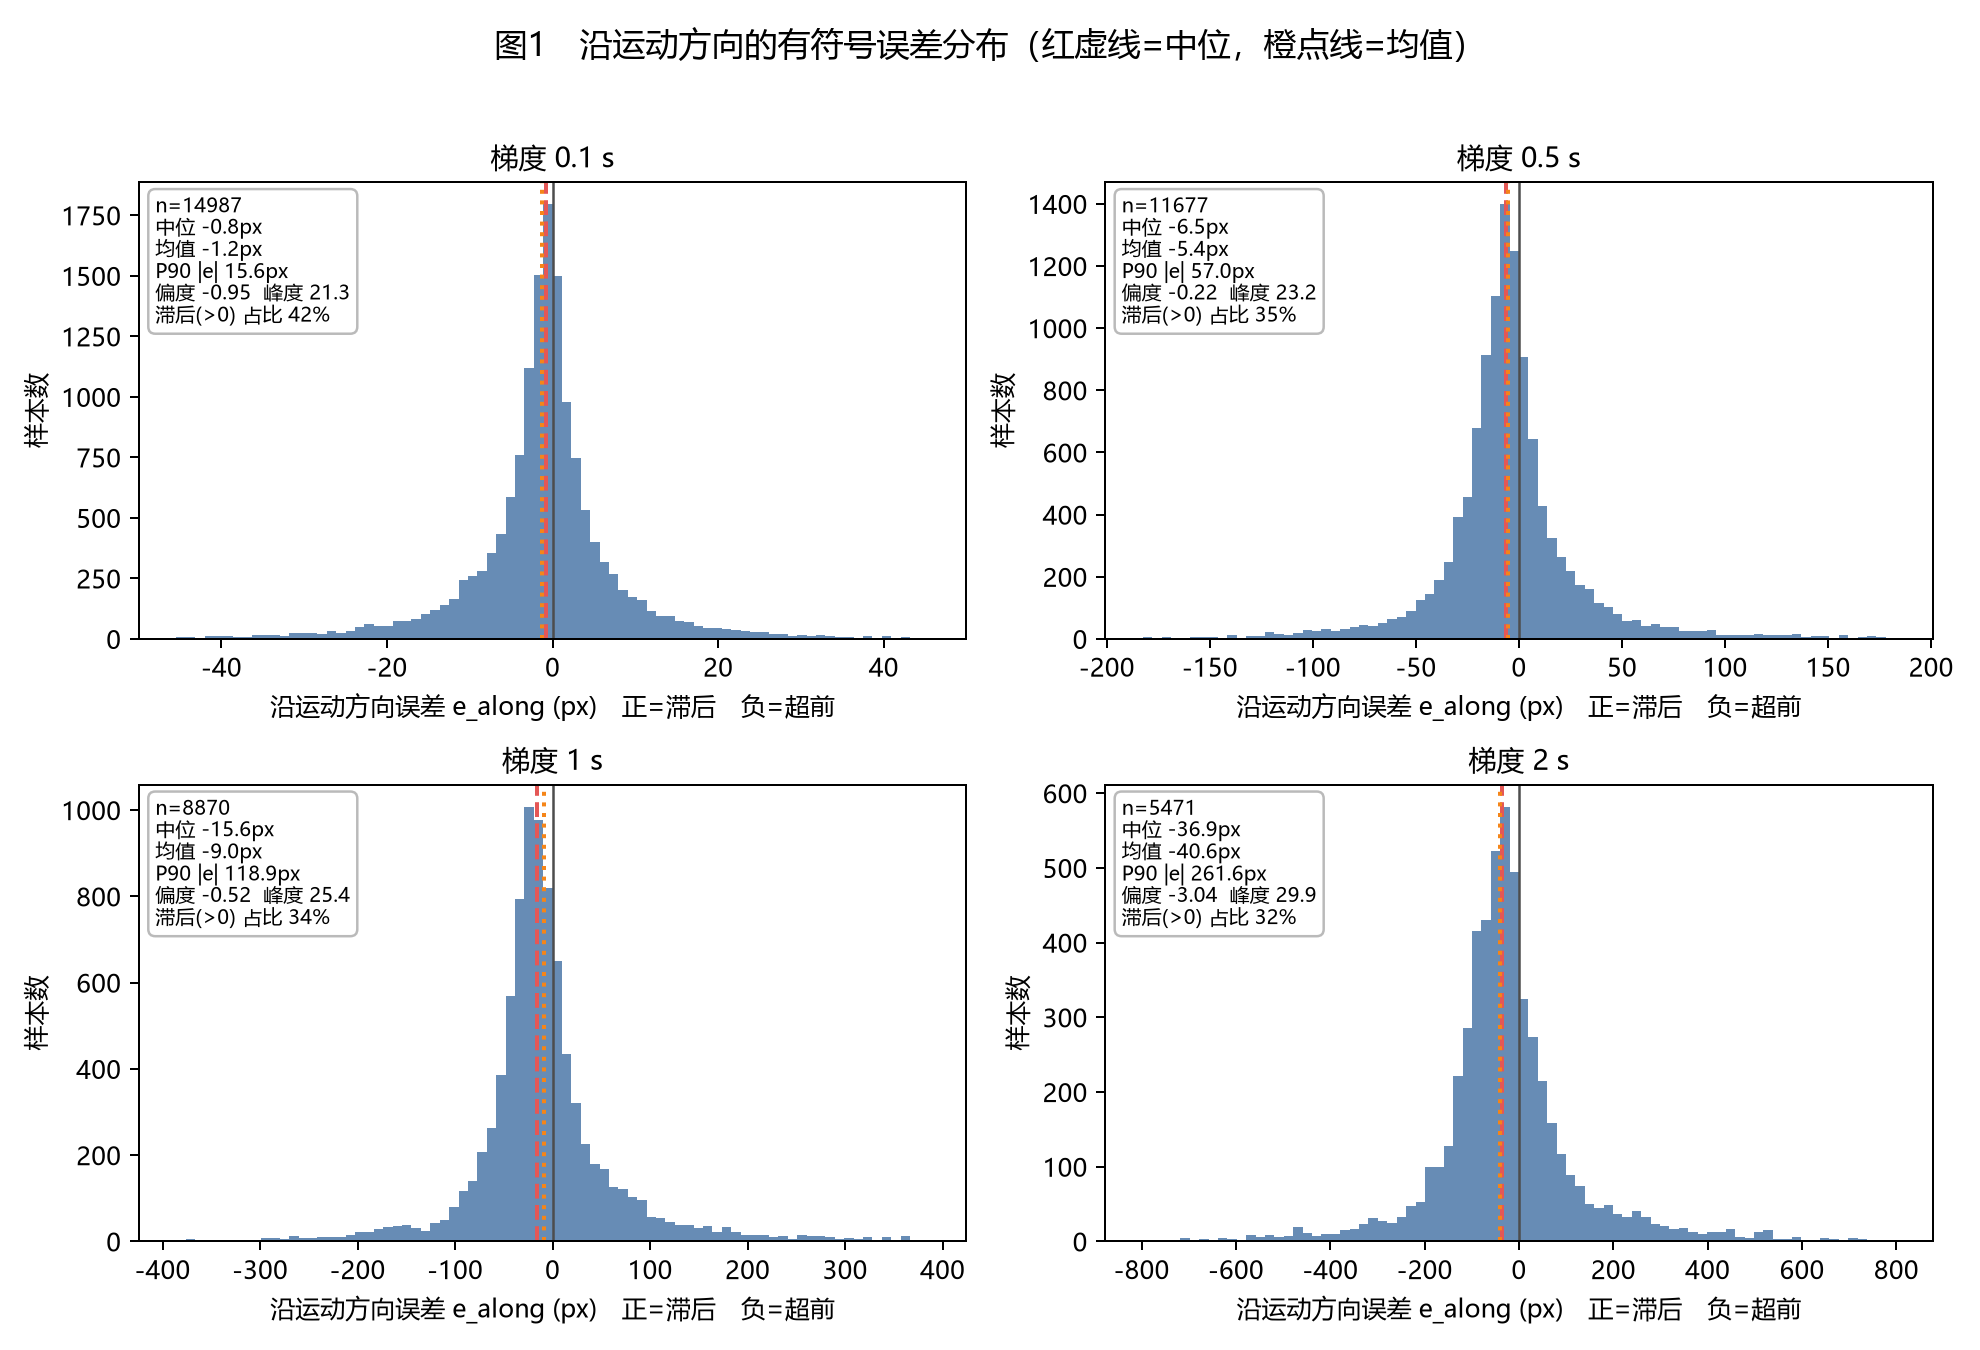
\includegraphics[width=\linewidth]{fig_signed_error_by_horizon.png}
\caption{各梯度沿运动方向的有符号误差分布。正值表示预判滞后（短打），负值表示
超调（长打）。四个梯度的中位偏置均为负且随梯度线性放大。}
\label{fig:signed}
\end{figure}

负号意味着\textbf{系统性超调}：只有 32\%$\sim$42\% 的样本滞后，其余都打过头。
进一步做带截距的标定拟合（把实测位移回归到预判位移上）：0.1$\sim$1 秒的斜率在
0.891$\sim$0.960 之间、截距接近 0（$+0.2$ 到 $-2.7$ 像素），说明偏差是\emph{乘性}的；
2 秒档斜率降到 0.633 而决定系数只剩 0.340，线性标定在 2 秒档已经失效。过原点增益
$g^\ast$ 分别为 0.899/0.940/0.921/0.711，但\textbf{把它套上去平均绝对误差只改善
0.55\%/2.50\%/2.47\%/3.41\%}（图\ref{fig:calib}）。这条结果的价值在于它是否证：
全局标定几乎不值钱。

\begin{figure}[t]\centering
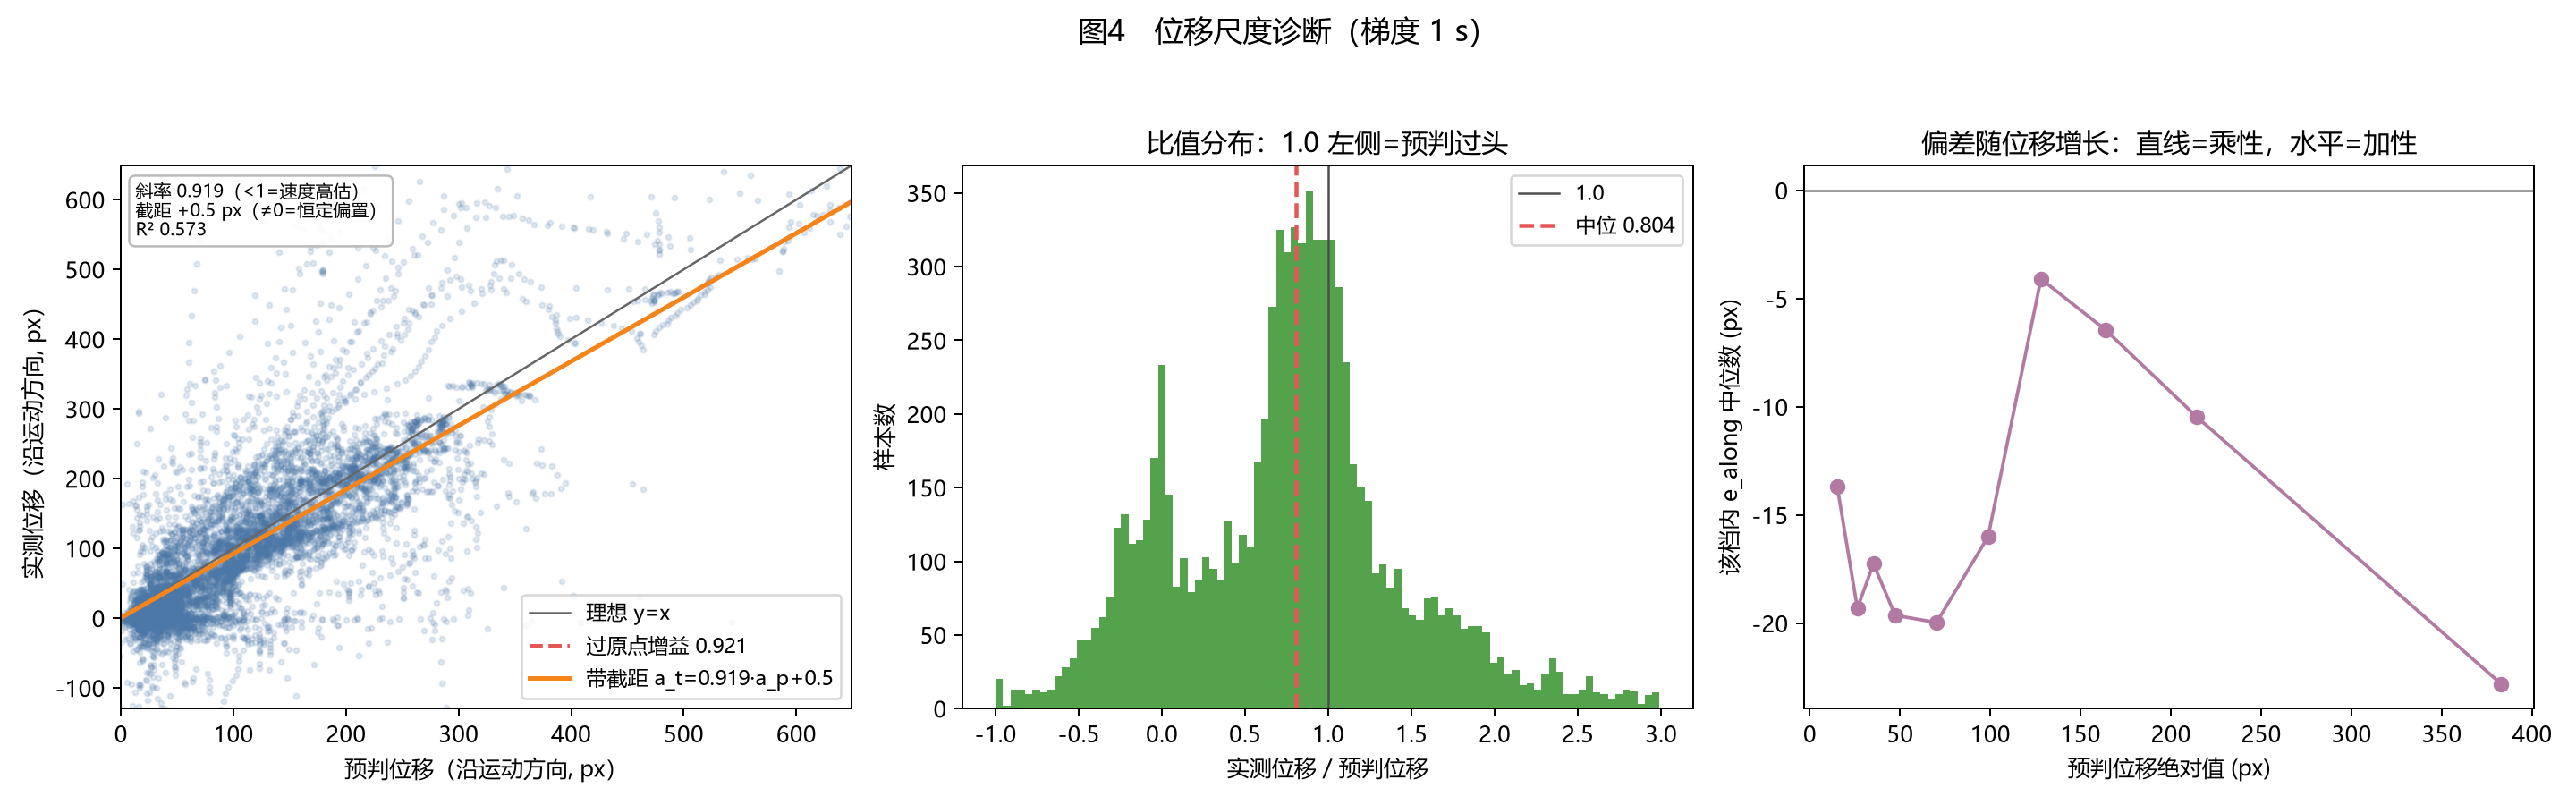
\includegraphics[width=\linewidth]{fig_displacement_calibration.png}
\caption{位移标定诊断。左：实测位移对预判位移的散点与两条拟合（过原点与带截距）；
中：实测与预判位移之比分布，中位 0.804 在 1.0 左侧；右：偏置随位移的走势。}
\label{fig:calib}
\end{figure}

那么偏置是"时间轴错位"还是"速度量级高估"？我们用等效时间偏置来判定：把像素偏差
除以目标自身速度。若是时间轴错位，该量应随梯度\emph{基本不变}；若是速度量级高估，
应随梯度\emph{线性增长}。实测为 $-0.008/-0.064/-0.170/-0.516$ 秒，明确属于后者
（图\ref{fig:offset}）。分类型看，标志牌的曲线几乎与 $y=h$ 重合——它的整段外推位移
都是错的，这引向下一节的尺度质疑。

\begin{figure}[t]\centering
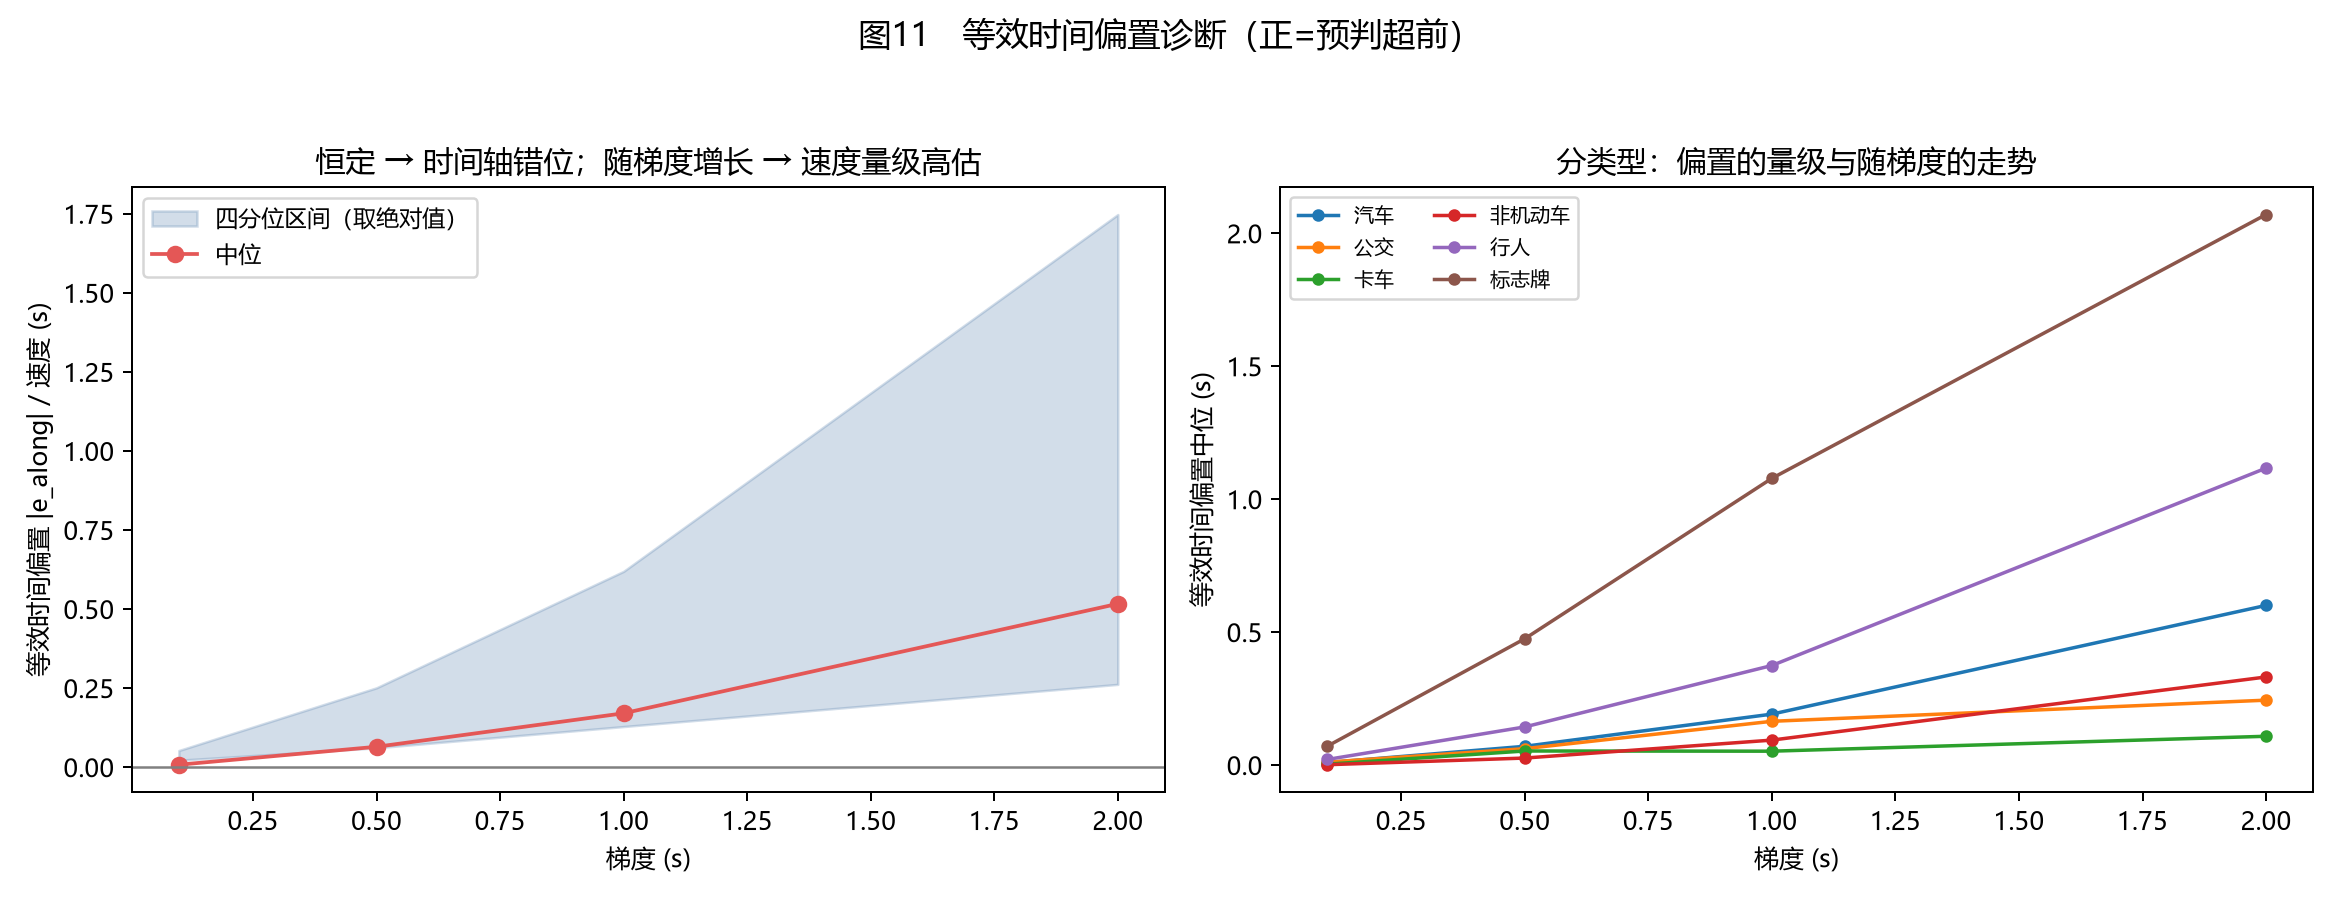
\includegraphics[width=\linewidth]{fig_equivalent_time_offset.png}
\caption{等效时间偏置（像素偏差除以目标速度）。中位随梯度线性增长，说明成因是速度
量级高估；标志牌的曲线接近 $y=h$，其外推位移整段失效。}
\label{fig:offset}
\end{figure}

\subsection{分布形态：不是高斯，也不是任何带折点的单峰族}

我们改用\emph{先估曲线、再定分布律}的顺序：先用高斯核密度（带宽做 0.05 到 0.40 的
扫描以排除带宽假象）在标准化尺度上估出密度，再看形状。

四条独立证据指向同一个方向。\textbf{(1) 对数密度}：|z| 落在 1$\sim$2.5 的斜率是
$-0.82$，2.5$\sim$4 的斜率是 $-0.53$，远尾比值 0.65$<$1，即\emph{远尾比近尾衰减更慢}。
近尾近指数、远尾重于指数，这正是尺度混合的特征（图\ref{fig:shape}）。\textbf{(2) 风险率}
$h(z)=f/S$ 在每一个类别上都是下降的，这是重尾分布的教科书指纹。\textbf{(3) 尾部}
实测拉普拉斯拟合的对数似然比高斯高出约 3078，但拉普拉斯仍罩不住尾部：
落在拟合分布 0.5\%/99.5\% 分位之外的实测比例高达 5\%$\sim$14\%，理想应为 1\%
（图\ref{fig:tail}）。\textbf{(4) 近峰质量}：mode 附近 $\pm0.1$ 稳健标准差内的实测
质量，汽车为 0.20，而高斯只给 0.08——实测峰比高斯尖出 2.5 倍。

\begin{figure}[t]\centering
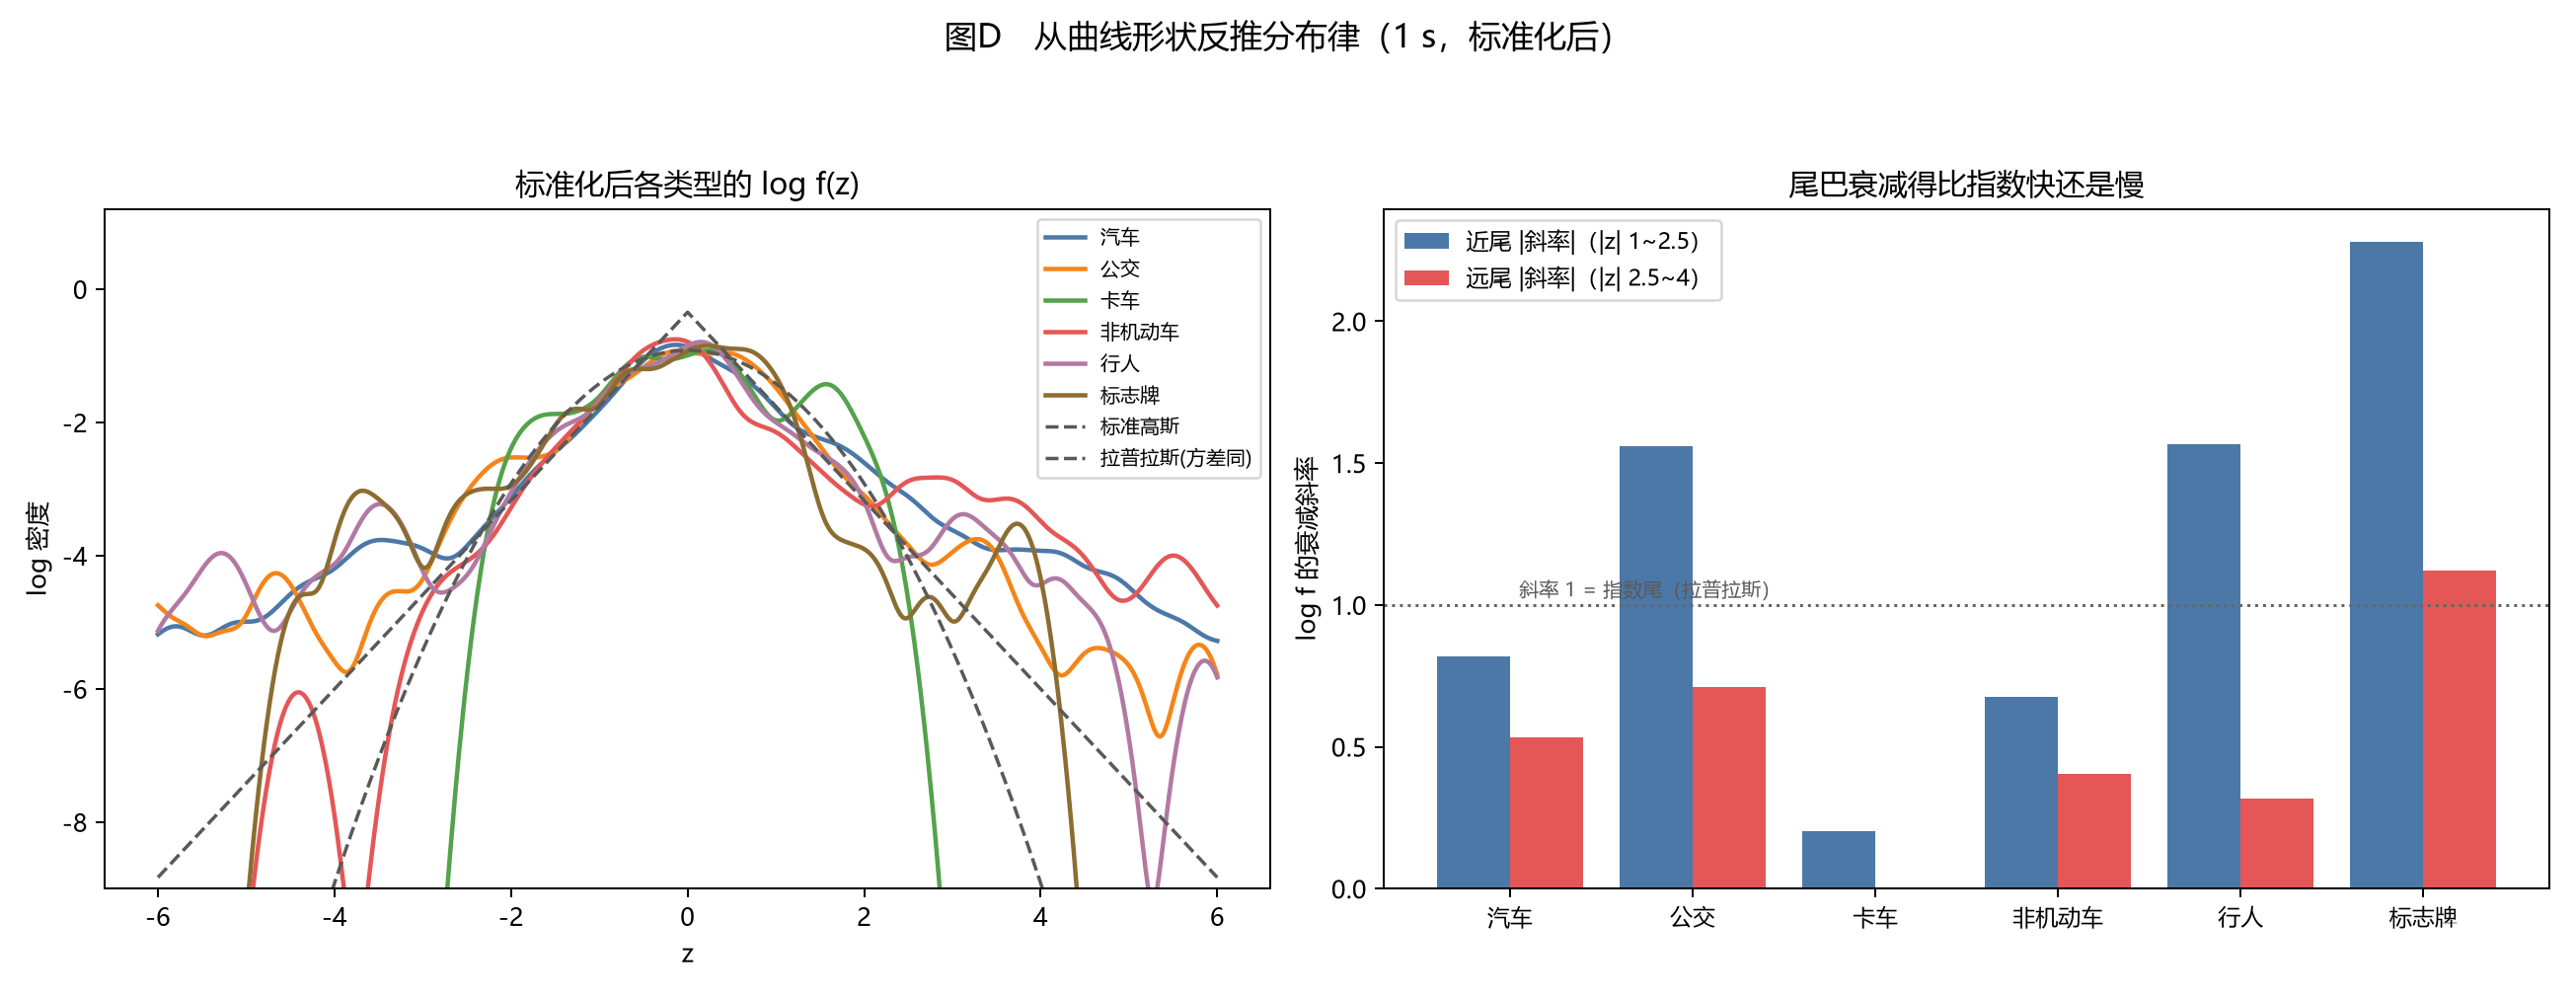
\includegraphics[width=\linewidth]{fig_shape_summary.png}
\caption{标准化后各类别的对数密度（左）与近尾、远尾的衰减斜率（右）。
斜率 1 对应指数尾；远尾斜率明显小于近尾，说明比指数尾更重。}
\label{fig:shape}
\end{figure}

\begin{figure}[t]\centering
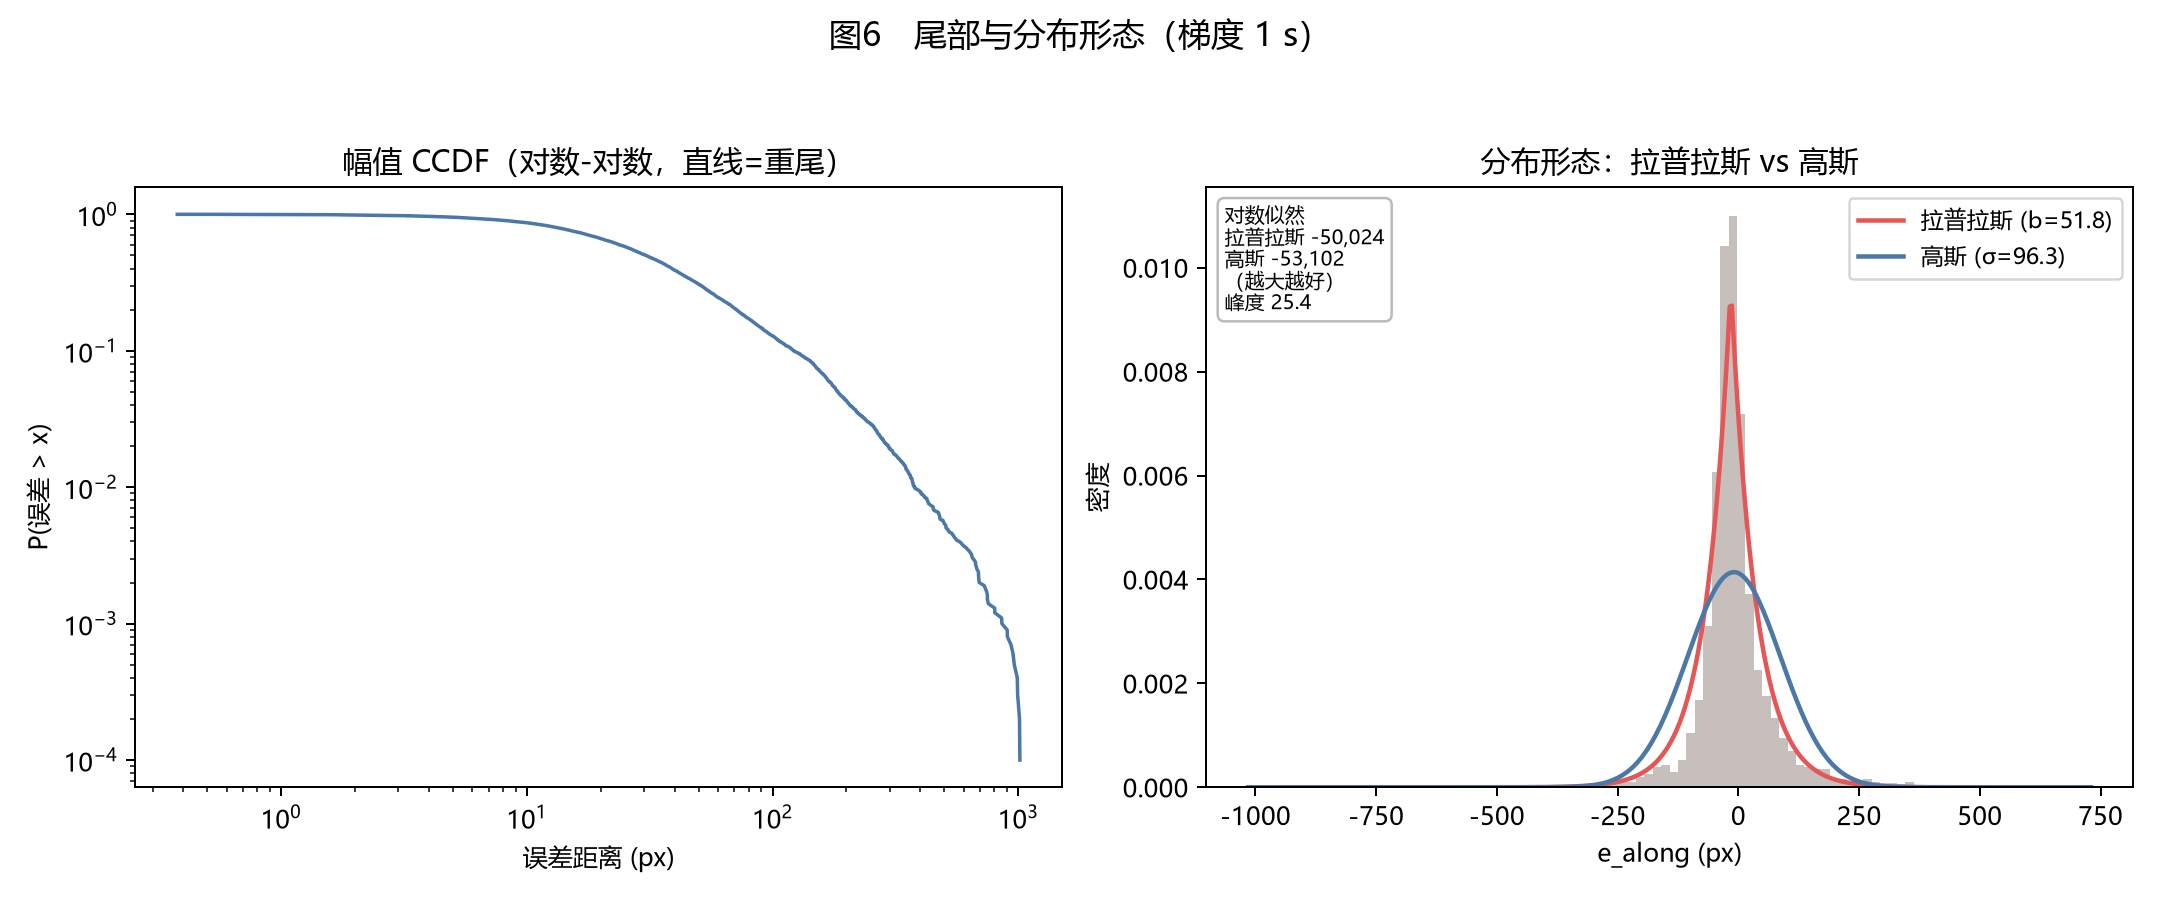
\includegraphics[width=\linewidth]{fig_tail_shape.png}
\caption{尾部形态。左：误差幅值的对数生存函数；右：有符号误差分布与拉普拉斯、
高斯拟合的对比。拉普拉斯在主体段贴合，但尾部仍偏轻。}
\label{fig:tail}
\end{figure}

把七个分布族放在一起做横评，结论非常干净（表\ref{tab:families}）。

\begin{table}[t]\centering\small
\caption{24 个"类别 $\times$ 梯度"单元格上的分布族胜出统计（胜出单元格数$_{\uparrow}$）。
BIC 为贝叶斯信息量准则，KS 为模型分布函数与经验分布函数的最大偏差；两者均以数值越小
为越优，"胜出"指该族在同一单元格上数值最小。平滑性一列说明该族密度函数是否存在
不可导点。}
\label{tab:families}
\begin{tabular}{llrr}
\toprule
分布族 & 平滑性 & BIC 胜出数$_{\uparrow}$ & KS 距离胜出数$_{\uparrow}$ \\
\midrule
学生 $t$ & 平滑 & 8 & 6 \\
两成分高斯混合 & 平滑 & 8 & \textbf{17} \\
不对称拉普拉斯 & 折点 & 4 & 1 \\
高斯 & 平滑 & 2 & 0 \\
拉普拉斯 & 折点 & 2 & 0 \\
两片高斯 & 折点 & \textbf{0} & \textbf{0} \\
偏正态 & 平滑 & \textbf{0} & \textbf{0} \\
\bottomrule
\end{tabular}
\end{table}

\textbf{带折点的两片高斯在 24 个单元格中一次都没有赢过}，偏正态同样一次没赢过；
稳定胜出的学生 $t$ 与两成分高斯混合恰好是同一件事的两面——\emph{尺度混合}。
近峰质量的判别更直接：两片高斯预测的近峰质量是 0.08，与高斯一样差，
\textbf{说明那个"尖点"是模型引进来的假象，数据里并不存在}。

\subsection{尺度混合：少数样本垄断方差}

既然分布是尺度混合，就把它显式拟合出来。表\ref{tab:mixture} 给出 1 秒档的分解。

\begin{table}[t]\centering\small
\caption{误差的尺度混合分解（1 秒档）。协议：先把误差除以框高以消除透视尺度，
再用期望最大化拟合两成分高斯混合，并取尺度较小的成分为主体；主体权重与尺度比
在四个梯度上的取值列于正文。}
\label{tab:mixture}
\begin{tabular}{lrrrrr}
\toprule
类别 & 样本数 & 主体权重 $w$ & 尺度比 $\sigma_2/\sigma_1$ & 尾部分量方差占比 \\
\midrule
汽车 & 5630 & 0.861 & 3.90 & 0.710 \\
非机动车 & 1595 & 0.718 & \textbf{7.27} & 0.950 \\
行人 & 528 & 0.749 & 6.56 & 0.940 \\
公交 & 772 & 0.766 & 3.27 & 0.770 \\
标志牌 & 209 & 0.640 & 2.82 & 0.820 \\
\bottomrule
\end{tabular}
\end{table}

主题权重在四个梯度上基本稳定（汽车 0.68$\rightarrow$0.79），尺度比略微放大
（4.8$\rightarrow$5.9 倍）——结构固定，只是两个尺度一起被梯度拉长
（图\ref{fig:mixture}）。这条结果统一解释了此前所有分散的观察：
\textbf{21\%$\sim$36\% 的样本贡献了 75\%$\sim$98\% 的总方差}。于是全局增益只值
2.5\%（它校正主体）、ALD 看着还行又不够（它只管主体段）、两片高斯全败
（单尺度加折点与"两条尺度"不是一回事）、尾部超额与集中度偏高——都是同一结构的
不同投影。

\begin{figure}[t]\centering
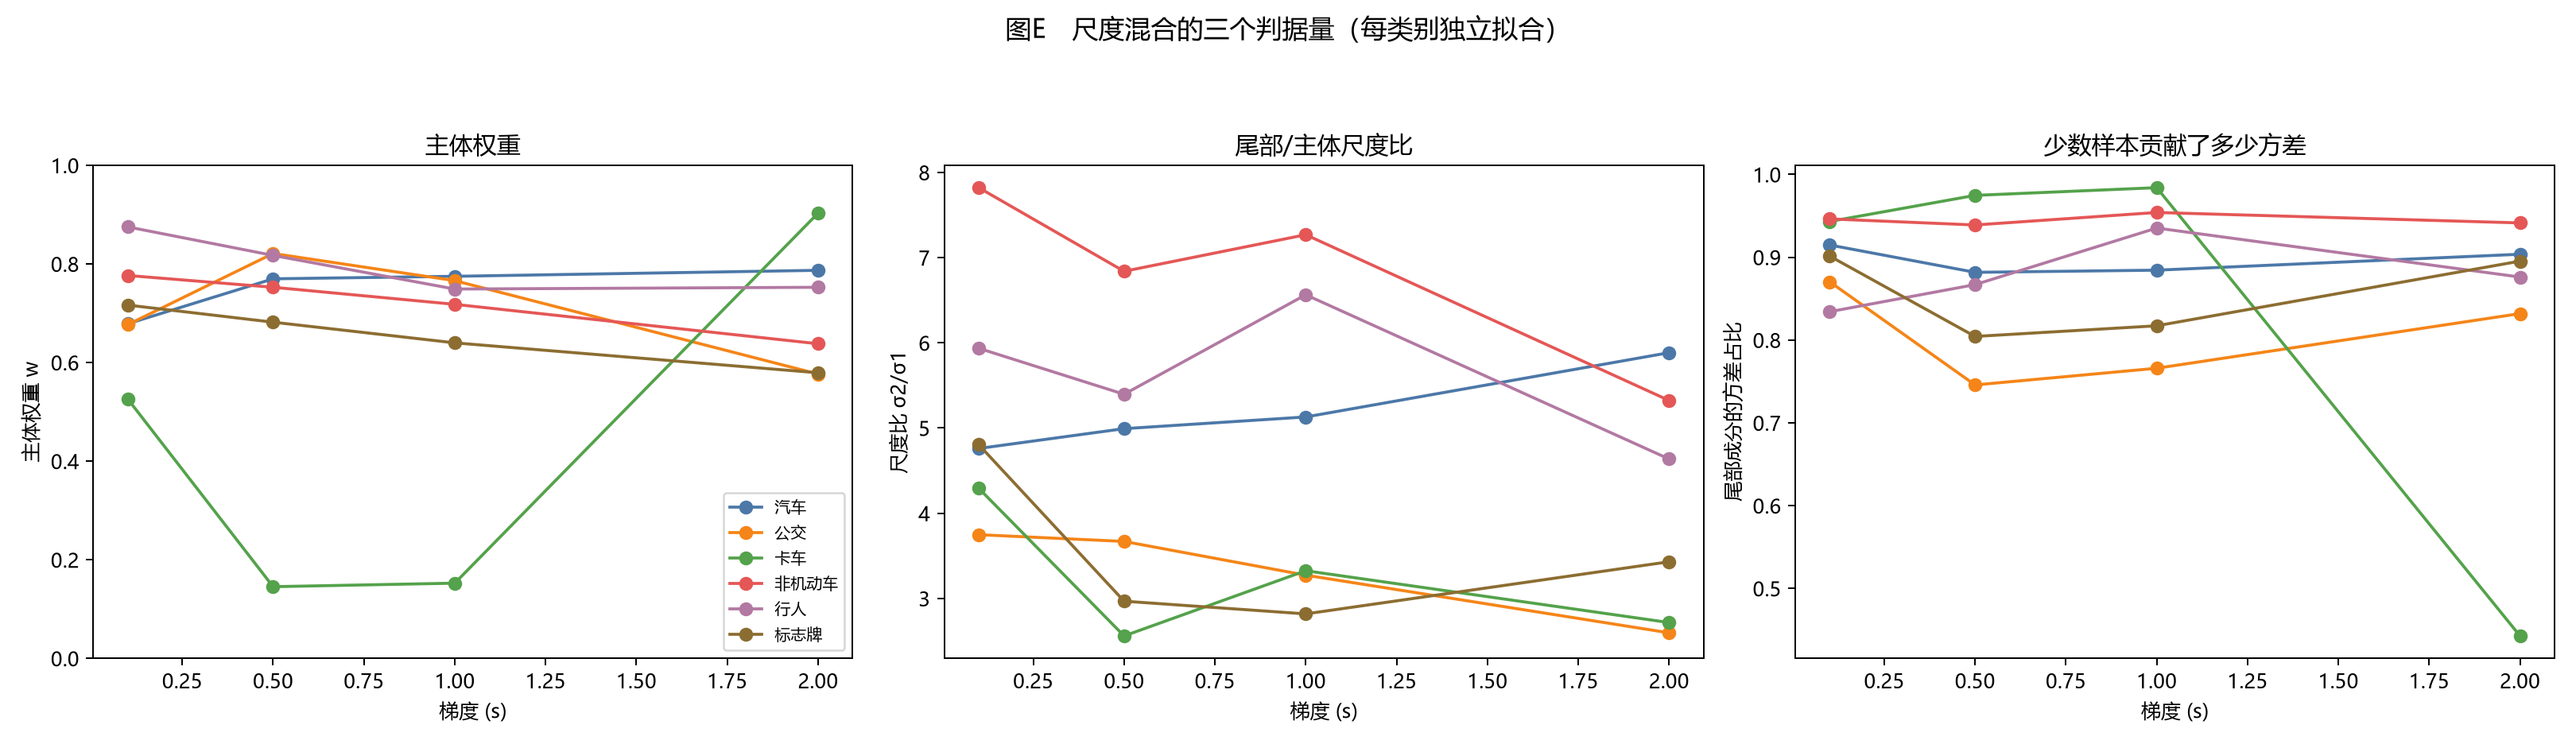
\includegraphics[width=\linewidth]{fig_scale_mixture_summary.png}
\caption{尺度混合的三个判据量随梯度的走向：主体权重、尺度比、尾部成分的方差占比。
每类别独立拟合。}
\label{fig:mixture}
\end{figure}

\subsection{尺度归一化对照：重尾不是透视假象}

在像素口径下，一个自然的怀疑是：所谓"重尾"不过是"近处目标像素误差天然大"。
我们做了两件事来检验。第一，把误差除以框高（预测时刻已知，且透视下像素位移与
目标像素尺寸成正比），得到尺度无关口径。第二，把两类尺度代理从门控特征里逐步剔除
（表\ref{tab:norm}）。

\begin{table}[t]\centering\small
\caption{尺度归一化对照。协议：标签取尺度无关口径下的重尾成员（后验责任大于 0.5），
特征只使用预测时刻已知的量，评估用留一视频交叉验证，一律用像素误差衡量。
曲线下面积与平均精度均以越高越好（$_{\uparrow}$）。}
\label{tab:norm}
\begin{tabular}{llrr}
\toprule
编号 & 设定 & 样本外 AUC$_{\uparrow}$ & 平均精度$_{\uparrow}$ \\
\midrule
A & 像素口径尾部标签，全部特征 & 0.769 & 0.430 \\
B & 像素口径尾部标签，去框高 & 0.726 & 0.362 \\
C & 归一化口径尾部标签，全部特征 & 0.753 & 0.448 \\
D & 归一化口径尾部标签，去框高 & 0.749 & 0.448 \\
E & 归一化口径尾部标签，去全部尺度代理 & 0.714 & 0.408 \\
\bottomrule
\end{tabular}
\end{table}

结论是清楚的。对数误差与对数框高的相关系数只有 0.192，\textbf{框高只解释误差方差的
3.7\%}；两个口径判定的重尾样本只有 12.5\% 不一致；框高在像素口径里值 0.043 的
AUC，归一化之后只剩 0.004；而\textbf{即使把全部尺度代理都拿掉，AUC 仍有 0.714}
（图\ref{fig:norm}）。因此重尾不是透视产物，剩下的可分性是真实的因果信号，
来源是转角速度、机动标记、检测置信度、遮挡续推、轨迹年龄、同帧目标数与类别。

\begin{figure}[t]\centering
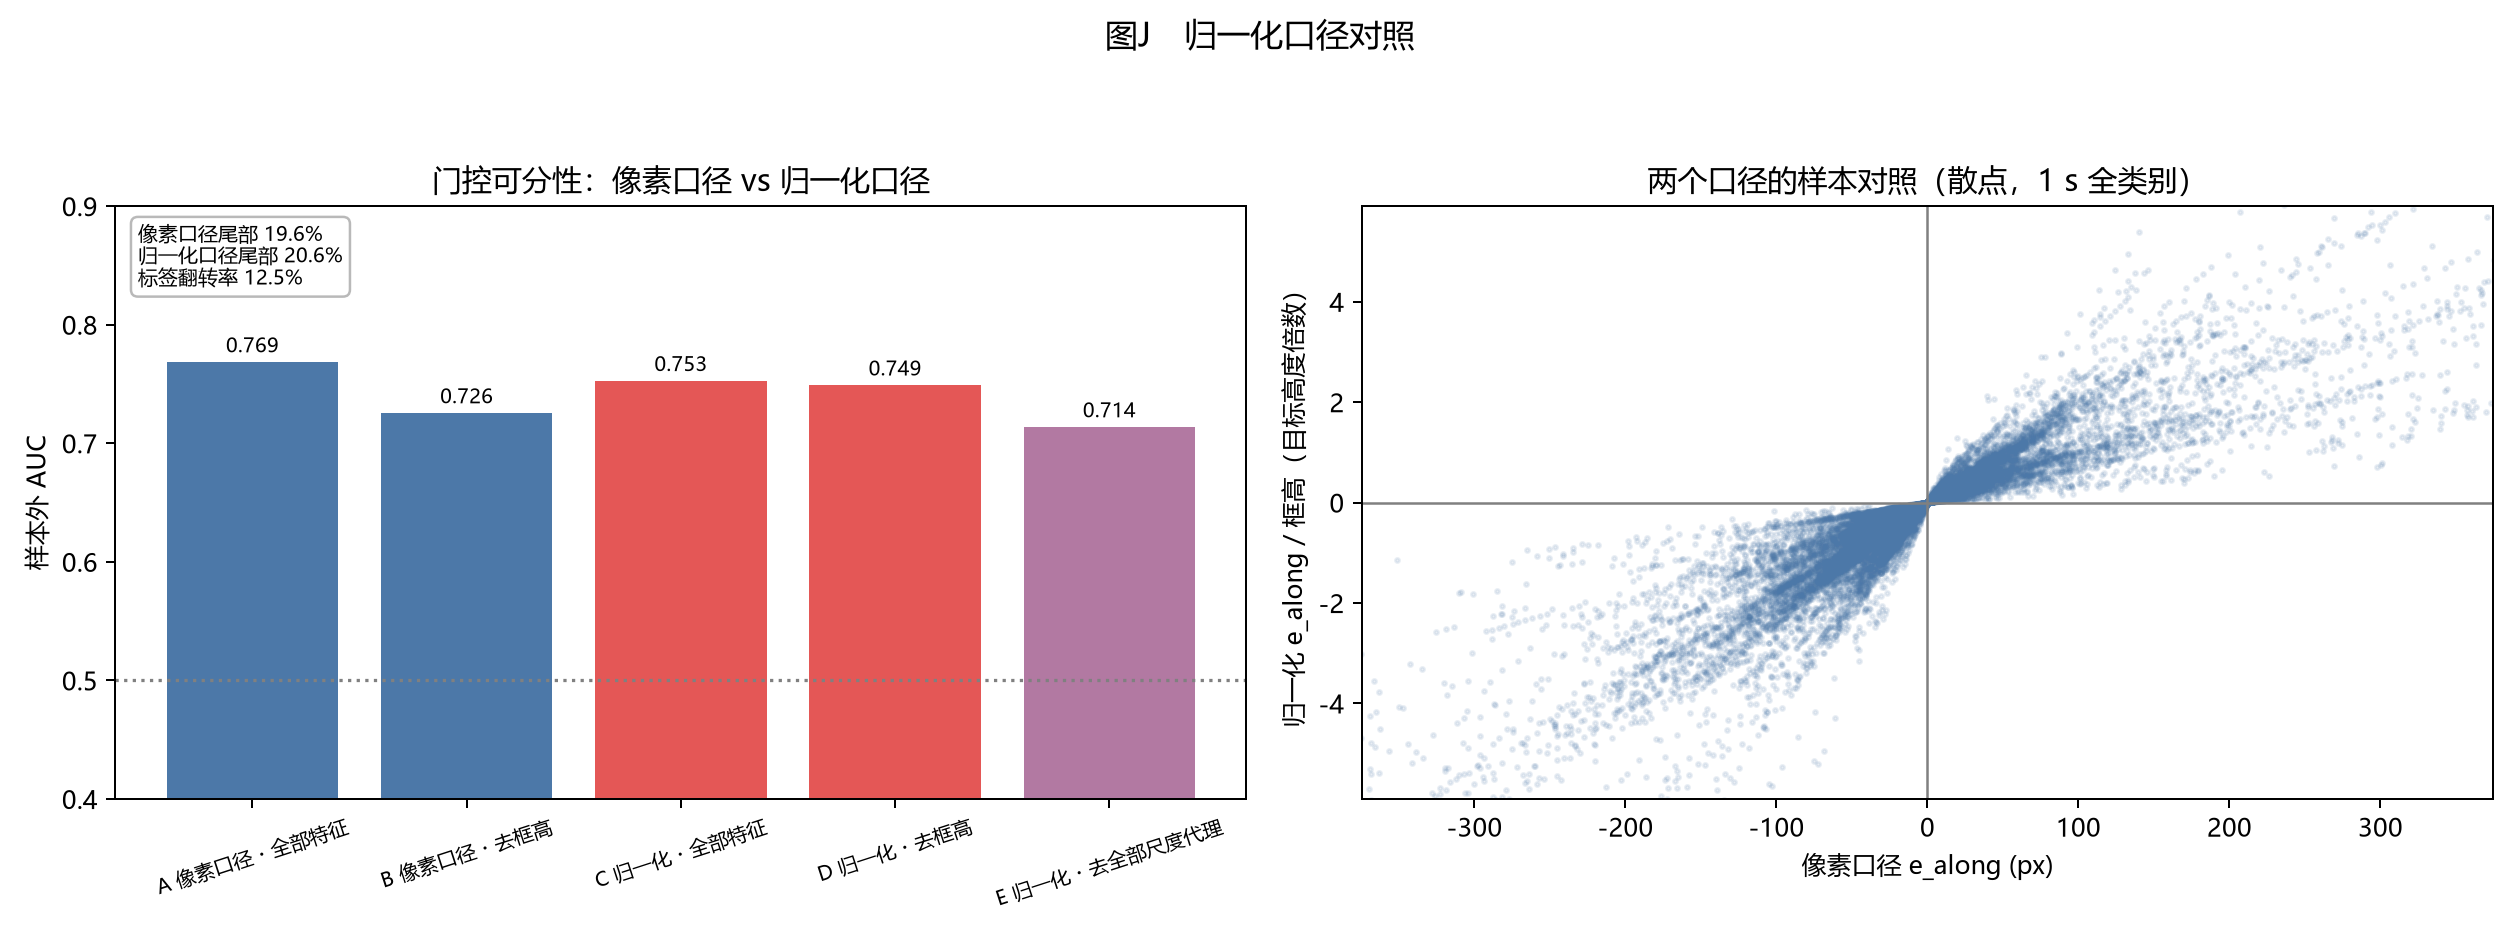
\includegraphics[width=\linewidth]{fig_normalisation_control.png}
\caption{尺度归一化对照。左：五个变体的样本外 AUC；右：两个口径下误差的散点对照。}
\label{fig:norm}
\end{figure}

\subsection{重尾样本的在线可分性，以及一条被推翻的结论}
\label{sec:gate}

既然重尾样本垄断方差，能否在\emph{事前}把它们捞出来并降级？我们以留一视频交叉验证
训练门控，标签为归一化口径下的重尾成员。可分性确实存在但不强：梯度提升样本外 AUC
0.767、平均精度 0.427（随机基线 0.196）。按类别看，行人 0.754、汽车 0.744、
卡车 0.717、非机动车 0.654、公交 0.550；标志牌只有 0.266，低于随机，属于污染源，
剥离后最弱项升到 0.550。

更难的是工作点：把查准率门槛从 0.4 提到 0.6，召回从 0.650 崩到 0.159
（图\ref{fig:gate}）。也就是说重尾成员不是一个能靠现有因果特征干净切出来的集合。
理想门控（用真实责任，需要未来）给出的上界是：中位从 14.1 降到 9.0 像素、
P90 从 94.3 降到 47 像素；而实际门控在保留 80\% 时只能把中位降到 11.7、
P90 降到 76——\textbf{它抓不住真正最差的那批，而 P90 恰恰是用户一眼会注意到的}。

\begin{figure}[t]\centering
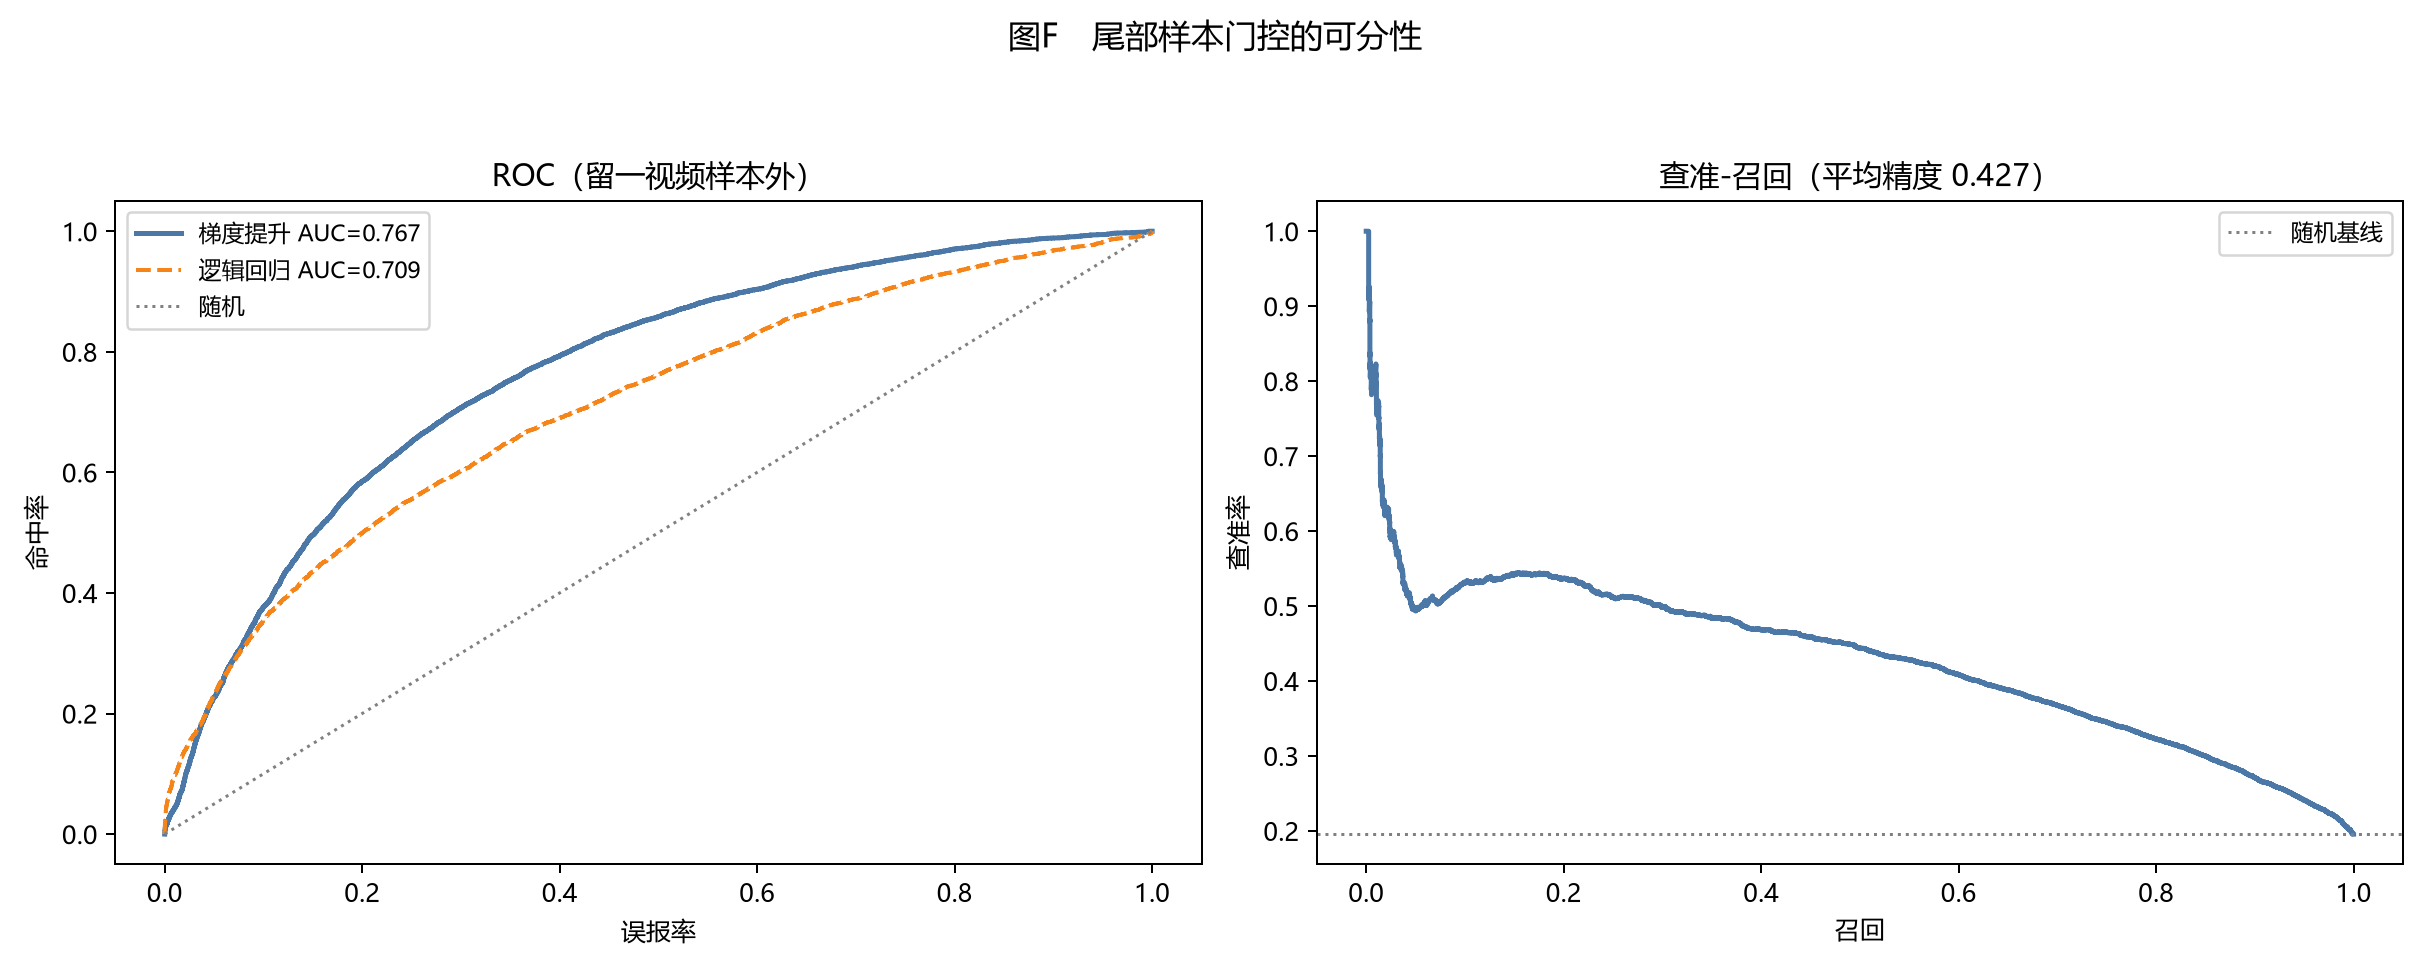
\includegraphics[width=0.92\linewidth]{fig_gate_roc_pr.png}
\caption{重尾标签门控的样本外 ROC 与查准-召回曲线（留一视频）。}
\label{fig:gate}
\end{figure}

这里必须报告一条我们\emph{自己推翻的结论}。最初的实验显示门控能把像素中位与
P90 各降 17\%$\sim$19\%，看起来很有价值。但把标签与特征做 $2\times2$ 拆解后发现：
像素口径下的收益主要来自"筛掉近处的大目标"——被标记样本的中位框高是 81.5 像素
（其余 48.5），中位误差 26.9 像素（其余 11.6），门控概率与框高的相关系数达 $+0.513$。
近处大目标恰恰是用户最关注的对象，把它们降级在指标上是划算的，在产品上是错的。
换成尺度无关标签后，同样门控标记出的样本中位误差是 13.8 像素，\emph{比未标记的
14.1 像素还小}；此时门控对像素指标不但无收益，在激进阈值下反而有害
（保留 50\% 时中位升到 17.6 像素）。因此我们撤回原先的乐观结论：
\textbf{在像素口径下，"用门控换精度"不成立}。

\begin{figure}[t]\centering
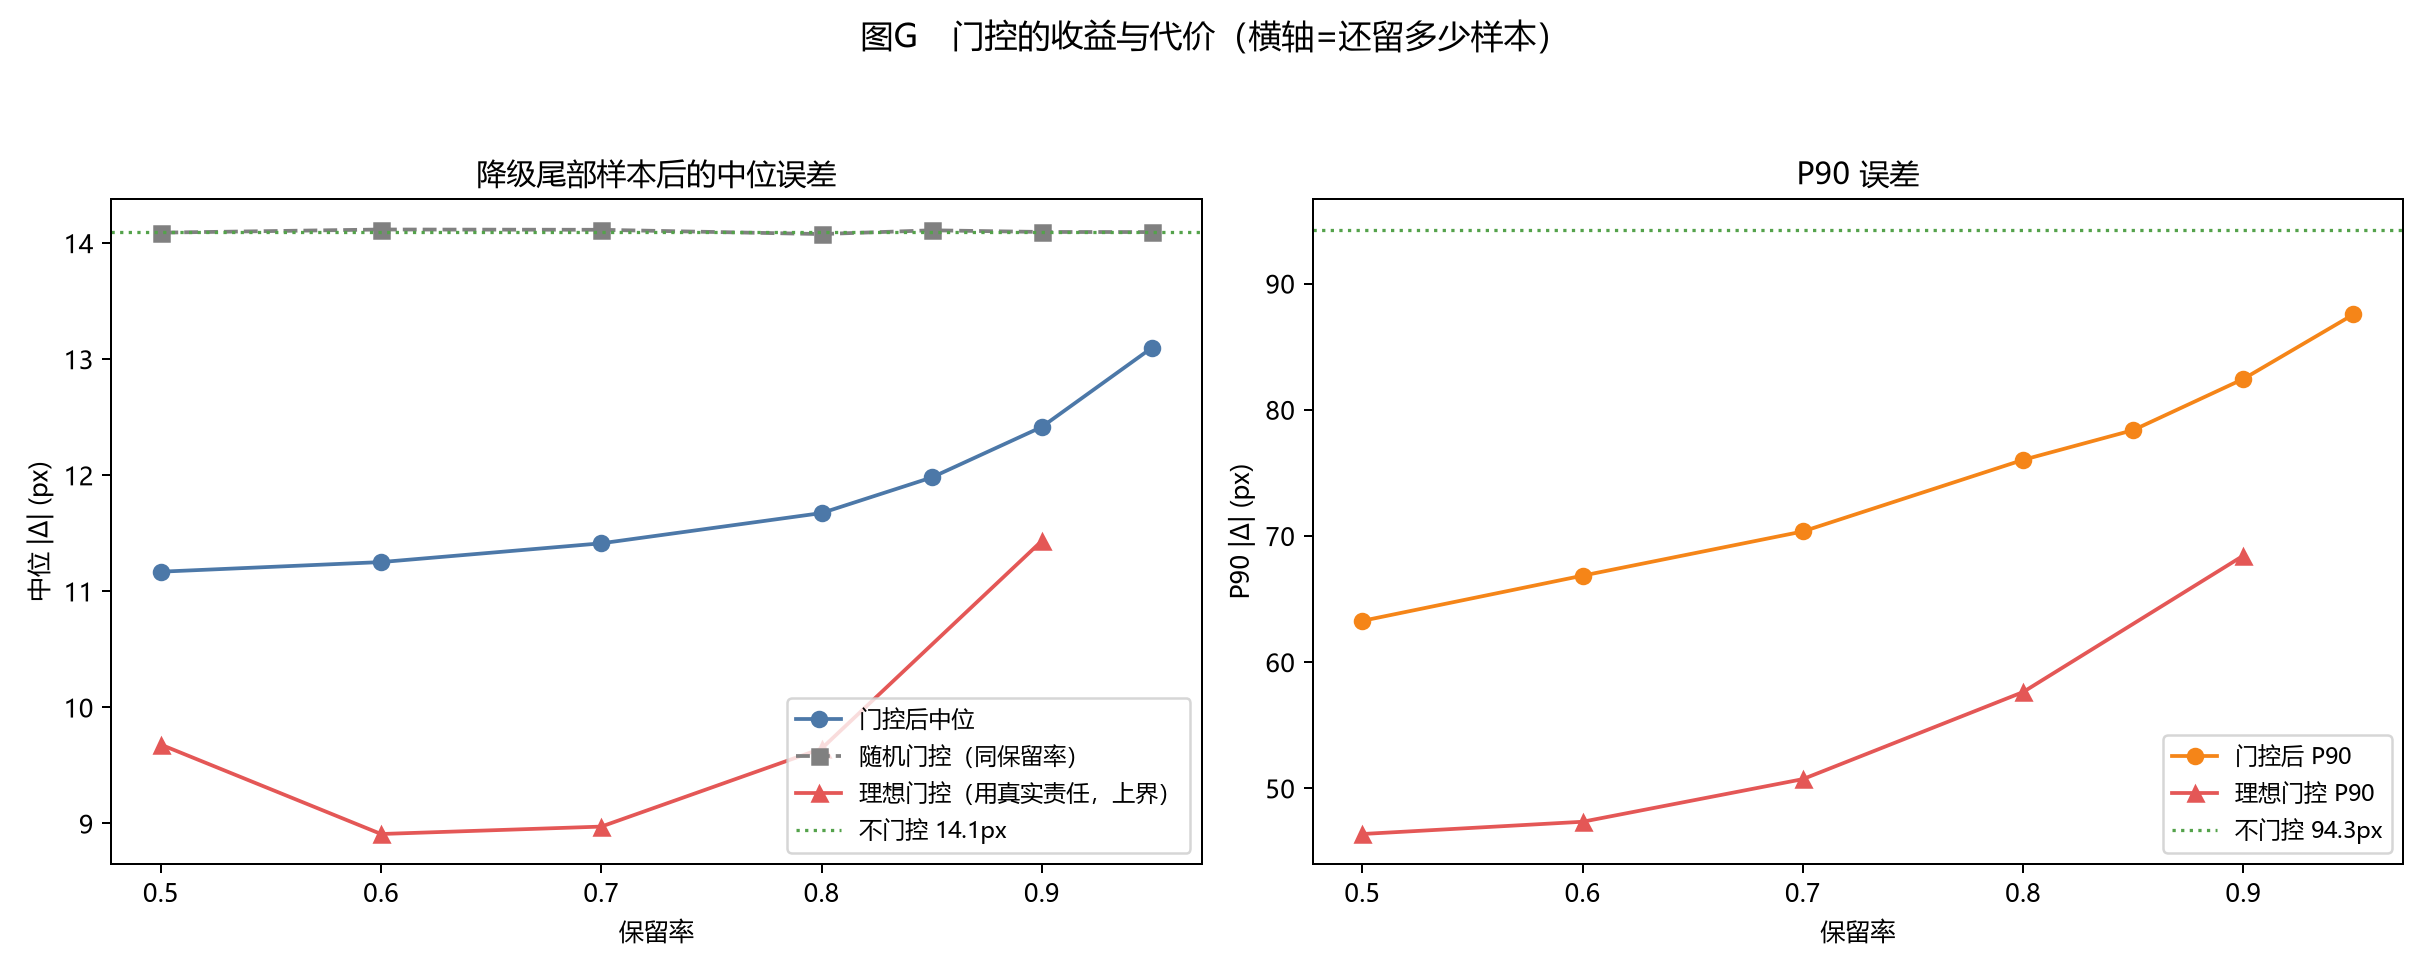
\includegraphics[width=0.92\linewidth]{fig_gate_benefit_cost.png}
\caption{门控的收益与代价。蓝线为实际门控，灰线为同保留率的随机门控，红线为使用
真实责任的理想门控上界。}
\label{fig:benefit}
\end{figure}

\subsection{像素口径下的误差归属与可控项}

验收口径定为像素误差，因此最后要回答的是：这 1.63\,M 像素的误差总量分布在哪里，
以及有哪些不牺牲覆盖的改动能把它压下去（表\ref{tab:attrib}）。

\begin{table}[t]\centering\small
\caption{像素误差质量的归属（四梯度合计）。协议：误差总量为全部样本的中心点距离之和
1.63\,M 像素，本表给出各归属的占比与中位误差；"机动样本"指转角速度超过判定阈值者，
"静态结构类"指标志牌与路桩。中位误差以越低越好（$_{\downarrow}$）。}
\label{tab:attrib}
\begin{tabular}{lrrr}
\toprule
归属 & 样本数 & 占误差总量 & 中位误差 (px)$_{\downarrow}$ \\
\midrule
汽车 & 27006 & \textbf{68.5\%} & 14.1 \\
非机动车 & 7033 & \textbf{17.8\%} & 12.7 \\
公交 & 3141 & 5.5\% & 14.4 \\
行人 & 2378 & 5.0\% & 14.9 \\
标志牌 & 813 & 1.6\% & 18.9 \\
卡车 & 619 & 1.5\% & 17.1 \\
\midrule
机动样本（转角超阈值） & 7755 & \textbf{30.1\%} & 22.5 \\
遮挡续推样本 & 3233 & 9.2\% & 23.4 \\
静态结构类 & 828 & 1.6\% & 18.6 \\
\bottomrule
\end{tabular}
\end{table}

关键读法是：\textbf{各类别的单位样本均值其实很接近（28$\sim$41 像素），总量差全在
样本数上}——汽车占 66\% 的样本。这一点决定了改进策略：个别类别的机制修复即使把
该类误差压掉八成，对总量也只有百分之几的影响。

我们用解析方式评估了最实在的一项机制修复：\textbf{静态结构零位移预判}
（预判框等于当前框，不外推）。由于垂直分量与预判无关（$\hat{u}\perp\hat{n}$），
新误差可以精确算出为 $\sqrt{a_{\text{true}}^2+e_{\text{cross}}^2}$。结果：标志牌
1 秒档中位从 31.9 降到 9.5 像素（$-70\%$）、P90 从 78.2 降到 30.6；2 秒档中位从
64.3 降到 10.6（$-84\%$）。但折算到全体只有 \textbf{$-1.01\%$} 的误差总量，
中位 14.1 到 13.6、P90 94.3 到 93.9（图\ref{fig:attrib}）。结论是：
\textbf{值得做，局部收益巨大且零成本，但它改不了大局}。

\begin{figure}[t]\centering
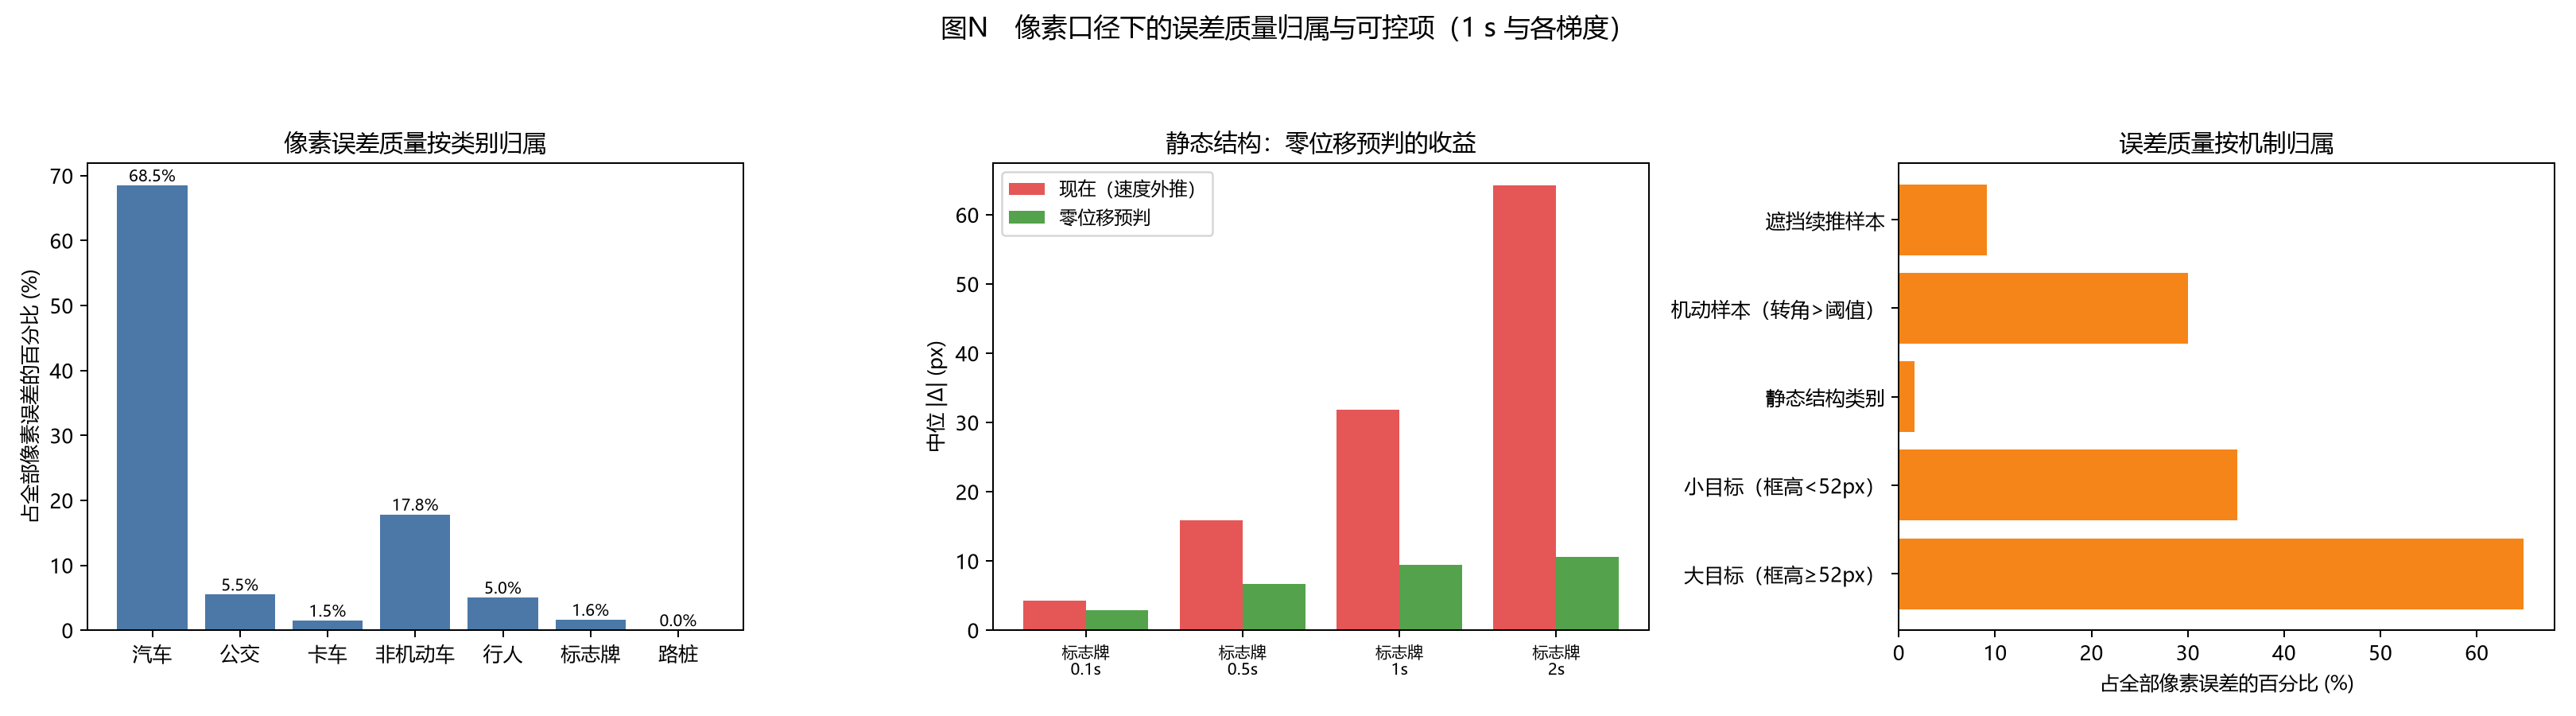
\includegraphics[width=\linewidth]{fig_error_attribution.png}
\caption{像素口径下的误差质量归属（左、右）与静态结构零位移预判的局部收益（中）。}
\label{fig:attrib}
\end{figure}

另一类是"不画预判框"的取舍：机动样本不给预判框时保留 81.1\%、中位降到 12.5、
P90 降到 82.5、均值降 13.8\%；再叠加续推样本则保留 74.1\%、均值降 15.5\%
（表\ref{tab:withhold}）。目标仍被检测与跟踪，只是明知不可靠就不外推。
我们认为画一个已知不可靠的框比不画更糟，但这是产品取舍而非技术结论。

\begin{table}[t]\centering\small
\caption{不画预判框这一取舍在保留率与像素误差之间的权衡。协议：被降级的样本仍然
被检测与跟踪，只是不输出预判框；保留样本为仍输出预判框的比例。保留率越高越好，
三种误差均以越低越好。}
\label{tab:withhold}
\begin{tabular}{lrrrr}
\toprule
策略 & 保留样本$_{\uparrow}$ & 中位 (px)$_{\downarrow}$ & P90 (px)$_{\downarrow}$ & 均值 (px)$_{\downarrow}$ \\
\midrule
基线（全画） & 1.000 & 14.1 & 94.3 & 39.8 \\
机动样本不画 & 0.811 & 12.5 & 82.5 & 34.3 \\
续推样本不画 & 0.921 & 13.2 & 93.3 & 39.3 \\
两者都不画 & 0.741 & 11.6 & 81.2 & 33.6 \\
\bottomrule
\end{tabular}
\end{table}

\section{负结果}
\label{sec:negative}

表\ref{tab:neg} 汇总了十一族被实测否掉的方案。我们把它当作与正结果同等重要的产出：
它把后续的改进预算从已经证否的方向上移开。需要说明，这些否掉的是\emph{在该设定下}
的收益，例如地面平面逆透视的失败源于我们没有真正的相机标定，而不是方法本身无效。

\begin{table}[t]\centering\small
\caption{已被实测否掉的技术路线。}
\label{tab:neg}
\begin{tabular}{p{0.26\linewidth}p{0.66\linewidth}}
\toprule
路线 & 实测结果 \\
\midrule
匀加速外推 & 比匀速差 3$\sim$8 倍（加速度估计被检测抖动主导） \\
圆弧外推（CTRV） & 阻尼转角扫描中 gain$=0$ 在每一档最优 \\
交互式多模型（IMM） & 8573 配对样本中仅 50\% 更准，中位/均值/P90 全面略差 \\
自适应卡尔曼（NIS 在线调 Q） & P90 从 116.6 恶化到 125.8 \\
地面平面逆透视（BEV） & 中位 34.6$\rightarrow$45.9、均值 57.7$\rightarrow$167.1；在该赢的深度变化档输得最多 \\
切图推理（SAHI 标准后处理） & 目标域 0.615$\rightarrow$0.600、旧街面 0.674$\rightarrow$0.634 \\
输入分辨率 1600 & 劣于 1280 \\
更大骨干（small） & 目标域 0.597 对 0.637，召回低 23\% \\
更换跟踪器（BoT-SORT、OC-SORT） & 同批目标中位误差仅差 1$\sim$3 像素，无工作点增益 \\
长关联缓冲 & 每帧可预判升到 12.11，但跳变从 72 翻倍到 149 次/千帧 \\
剔除静止类目标 & 指标反而更差 \\
\bottomrule
\end{tabular}
\end{table}

\section{讨论与局限}
\label{sec:discussion}

\textbf{算法收益已接近枯竭。}像素口径下，确定可得的机制收益只有：静态零位移
$-1.0\%$ 总量、全局增益 $-0.7\%$、机动门控 $-13.8\%$ 均值（代价 18.9\% 目标无预判框）。
而误差大头（汽车 68.5\%、机动样本 30.1\%）落在已经系统证否的技术路线里。这与
Sch\"oller 等在短时域上的结论一致 \citep{scholler2020cv}：不是实现水平问题，
而是任务在短时单目设定下的客观规律。

\textbf{数据是唯一还没被证否的方向。}非机动车贡献 17.8\% 的误差量却只有 7033 个
样本，卡车只有 619 个；更根本的是，本文全部预判误差的真值取自同一跟踪器的未来观测，
属于自证式测量，只反映"相对自身观测的一致性"。换成独立人工真值有可能改变
上述所有数值——包括尺度混合的权重。

\textbf{局限性。}第一，真值自证式，且只评中心点距离、未评框的重叠度。第二，六段
视频的样本量使留一交叉验证的置信区间较宽，分类型 AUC 中卡车（619 样本）与标志牌
（813 样本）的结论不稳。第三，标志牌的混合拟合本身不稳定（归一化 AUC 低于随机），
我们只能把它从统计中剔除，而不能给出它的正确描述。第四，本文的静态结构通道依赖
开放词汇检测与图文匹配，其依赖链的许可证为 AGPL-3.0，闭源交付需替换该环节。
第五，我们只验证了短时域（不超过 2 秒）；更长时间跨度上的结论不能外推。

\section{应用落地路径}
\label{sec:deploy}

本文交付的是一个批处理器，不是流式服务；距离实际部署还有四步，每一步都有实测依据。

\subsection{实时化}

端到端代价为 0.24\,s/帧，单张 8\,GB 显卡约合 4 帧/秒——足以处理已录制的片段，
跟不上直播流。开销结构是清楚的：主导项是开放词汇静态通道（318\,ms/帧），
场景先验把它降到 81\,ms/帧，于是同一段 816 帧素材的处理时间从约 4 分钟降到约 1 分钟；
剩余开销是 1280 分辨率下的检测（17$\sim$24\,ms/帧）。因此实时化的正确方向是
\textbf{调度}而非\textbf{容量}：在部分帧上降分辨率检测、再对可疑目标精细化，
而不是换更大的骨干——后者已被实测否掉（表\ref{tab:neg}）。这也解释了为什么
场景先验在本系统里不只是加速技巧，而是把"每段视频重付一次静态扫描成本"变成
"每个机位只付一次"的部署前提。

\subsection{一次相机标定换取米制速度}

当前输出只有像素。已安装的交通相机机位通常是固定的，因此一次标定即可把预判换算为
米与千米每小时，并解锁此前被我们否掉的地面平面建模
\citep{rezaei2021trafficnet,hirano2023vipm}。我们把这一项列为落地优先级最高，
理由是它\emph{新增}一个输出（真实速度）而不是改善一个已有输出：在像素口径的算法
收益已接近枯竭的前提下（第\ref{sec:analysis}节），这是性价比最高的一步，
而且它把系统的价值叙事从"框画得更准"换成"输出可直接用于限速与冲突预警的物理量"。

\subsection{合规、隐私与真值}

检测与关联链路是 AGPL-3.0，闭源交付必须替换为宽松许可的检测器与自研跟踪器；
该路径已做过可行性评估，属工程工作量而非研究风险。公开任何素材之前须完成人脸与
车牌脱敏，第三方航拍数据只提供转换脚本而不再分发原始图像 \citep{zhu2022visdrone}。

最后一条最重要，也最容易被跳过：本文全部预判数字都以同一跟踪器的未来观测为真值，
它衡量的是自洽性而非正确性。独立人工真值是唯一可能改变全部报数的输入——
可能变好也可能变坏——因而是把"精度"从内部一致性升级为可核验主张的唯一前提。
在没有它之前，本文的结论应当被理解为\emph{结构性的}（误差长什么样、错在哪一侧、
哪些路线无效），而不是\emph{绝对精度的}。

\section{结论}
\label{sec:conclusion}

我们交付了一个可在单张 8\,GB 显卡上运行的单目交通视频短时预判系统，规范口径下
目标域检测 mAP50 0.637、每帧可预判 14.87 个目标、1 秒预判中位误差 33.4 像素。
更重要的结论是误差的\emph{结构}：误差几乎全部沿运动方向、以系统性超调为主、
等效时间偏置随梯度线性增长；其分布是尺度混合而非任何带折点的单峰族，
由 21\%$\sim$36\% 的样本贡献 75\%$\sim$98\% 的方差。据此我们给出 $w$ 与
$\sigma_2/\sigma_1$ 两个判据量，并证明在像素口径下事后门控换不来精度。
最后，十一族替代方案被逐一实测并否掉。后续工作只剩下两条尚未被证否的路径：
用独立人工真值替换自证式真值，以及在固定机位下做真正的相机标定以获得米制速度与
可用的地面平面建模。

\clearpage
\bibliographystyle{plainnat}
\bibliography{refs}

\clearpage
\appendix
\section{补充图表}

\begin{figure}[h]\centering
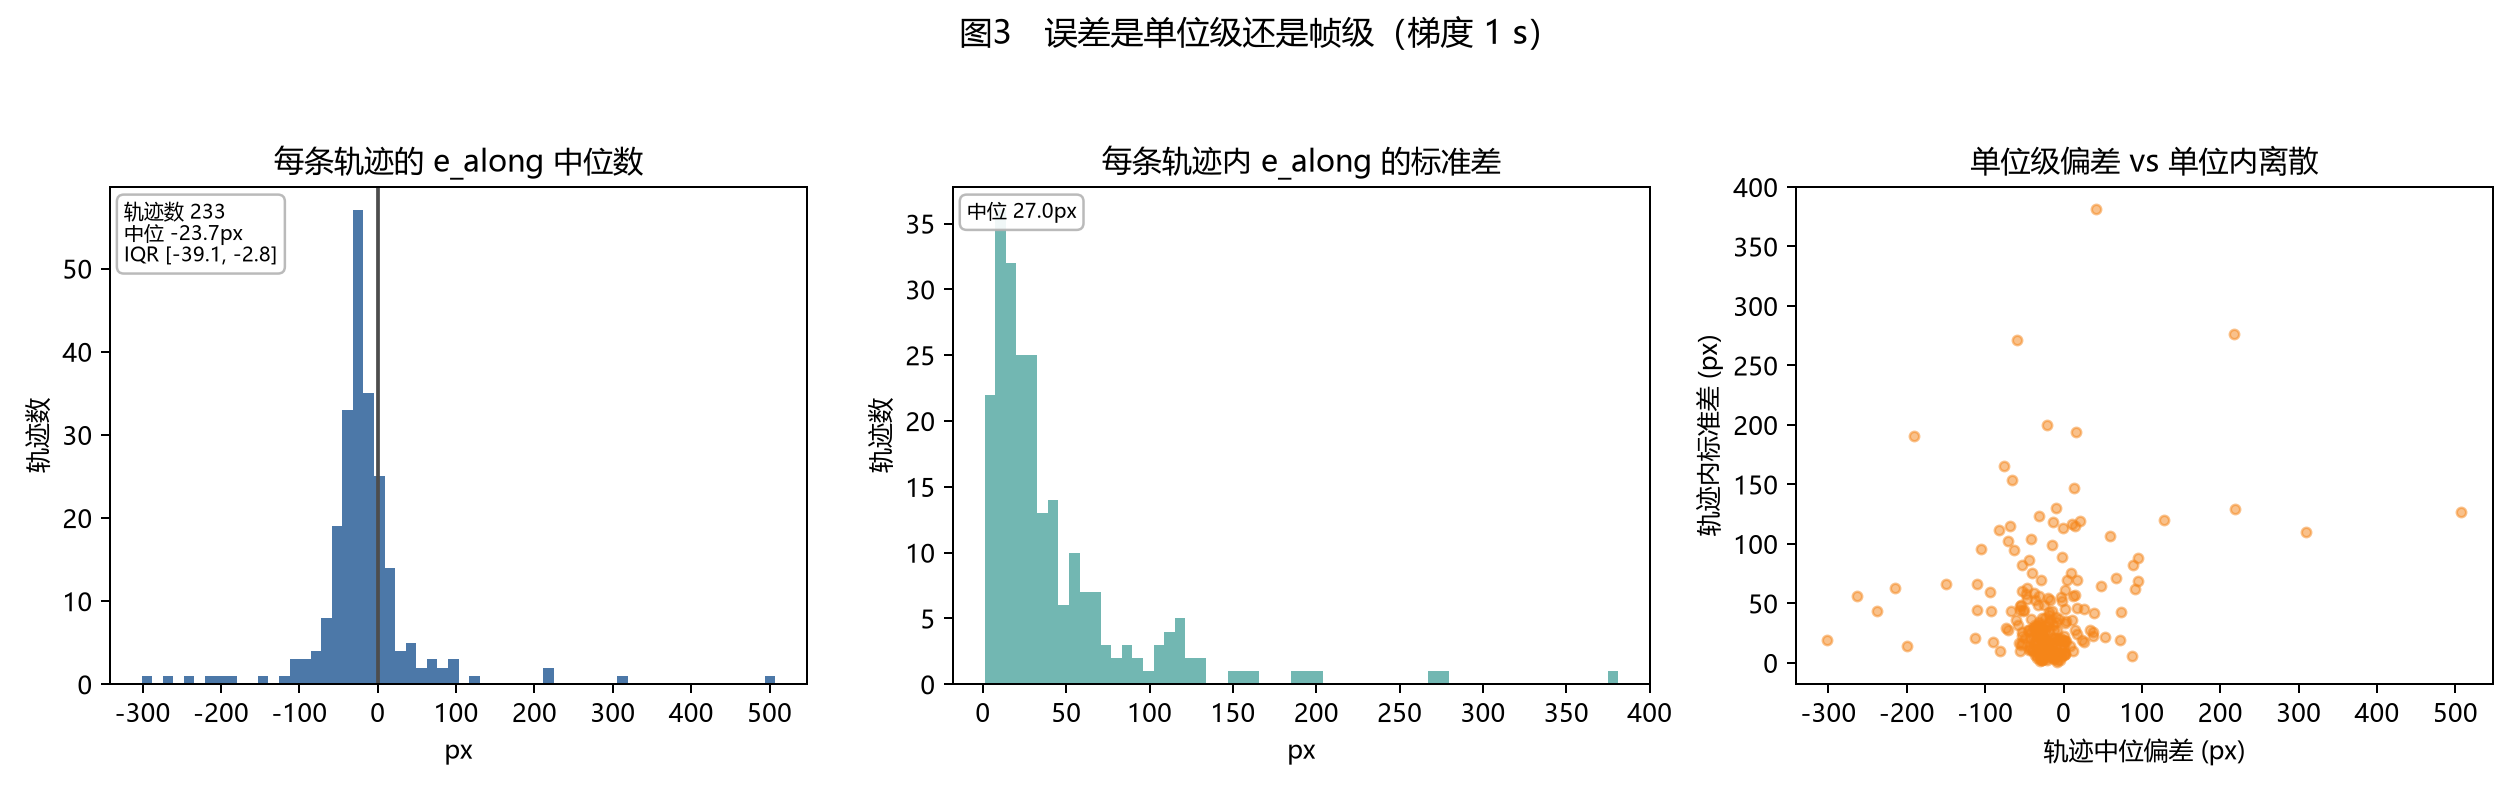
\includegraphics[width=0.92\linewidth]{fig_unit_vs_frame_error.png}
\caption{轨迹级与帧级误差分解，用于判断误差是单位级系统偏差还是帧级噪声。}
\end{figure}

\begin{figure}[h]\centering
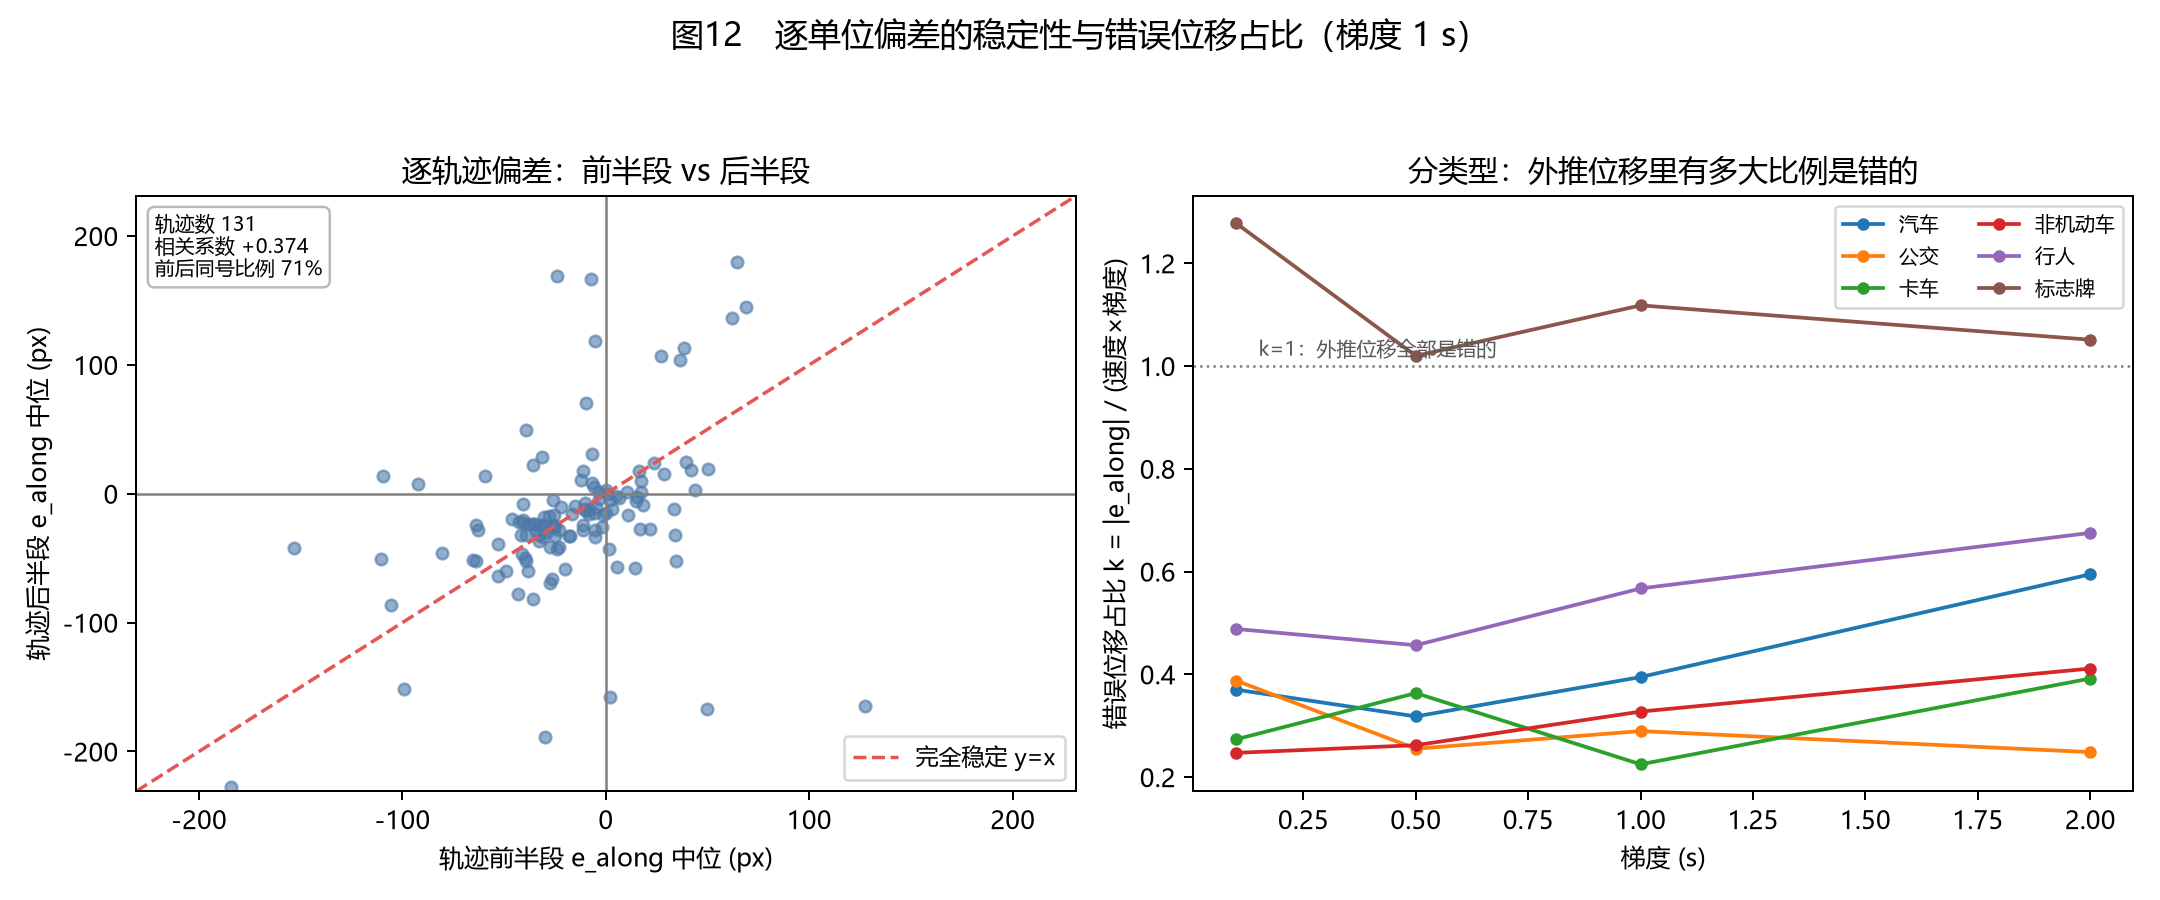
\includegraphics[width=0.92\linewidth]{fig_bias_persistence.png}
\caption{逐单位偏差在时间上的稳定性与分类型错误位移占比。}
\end{figure}

\begin{figure}[h]\centering
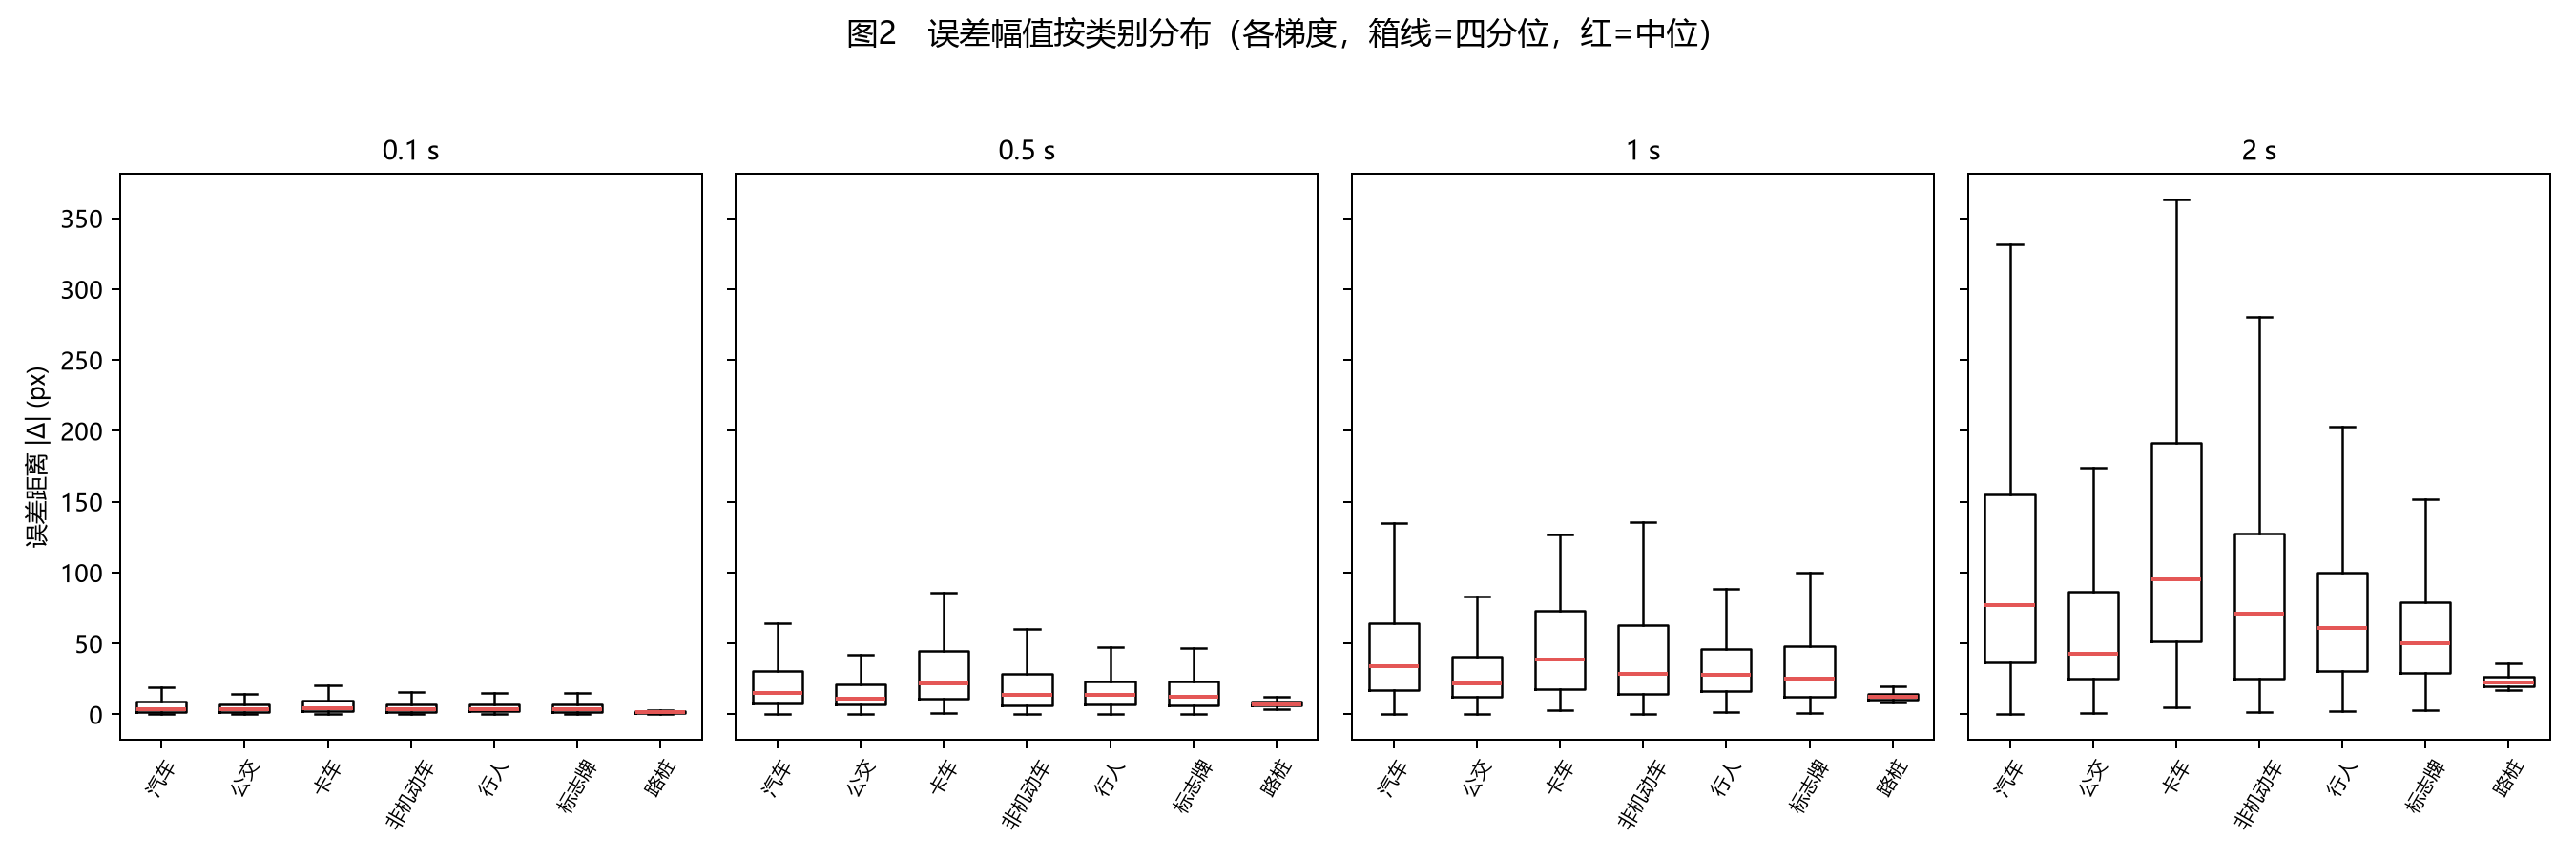
\includegraphics[width=0.92\linewidth]{fig_error_magnitude_by_class.png}
\caption{误差幅值按类别与梯度的分布。}
\end{figure}

\begin{figure}[h]\centering
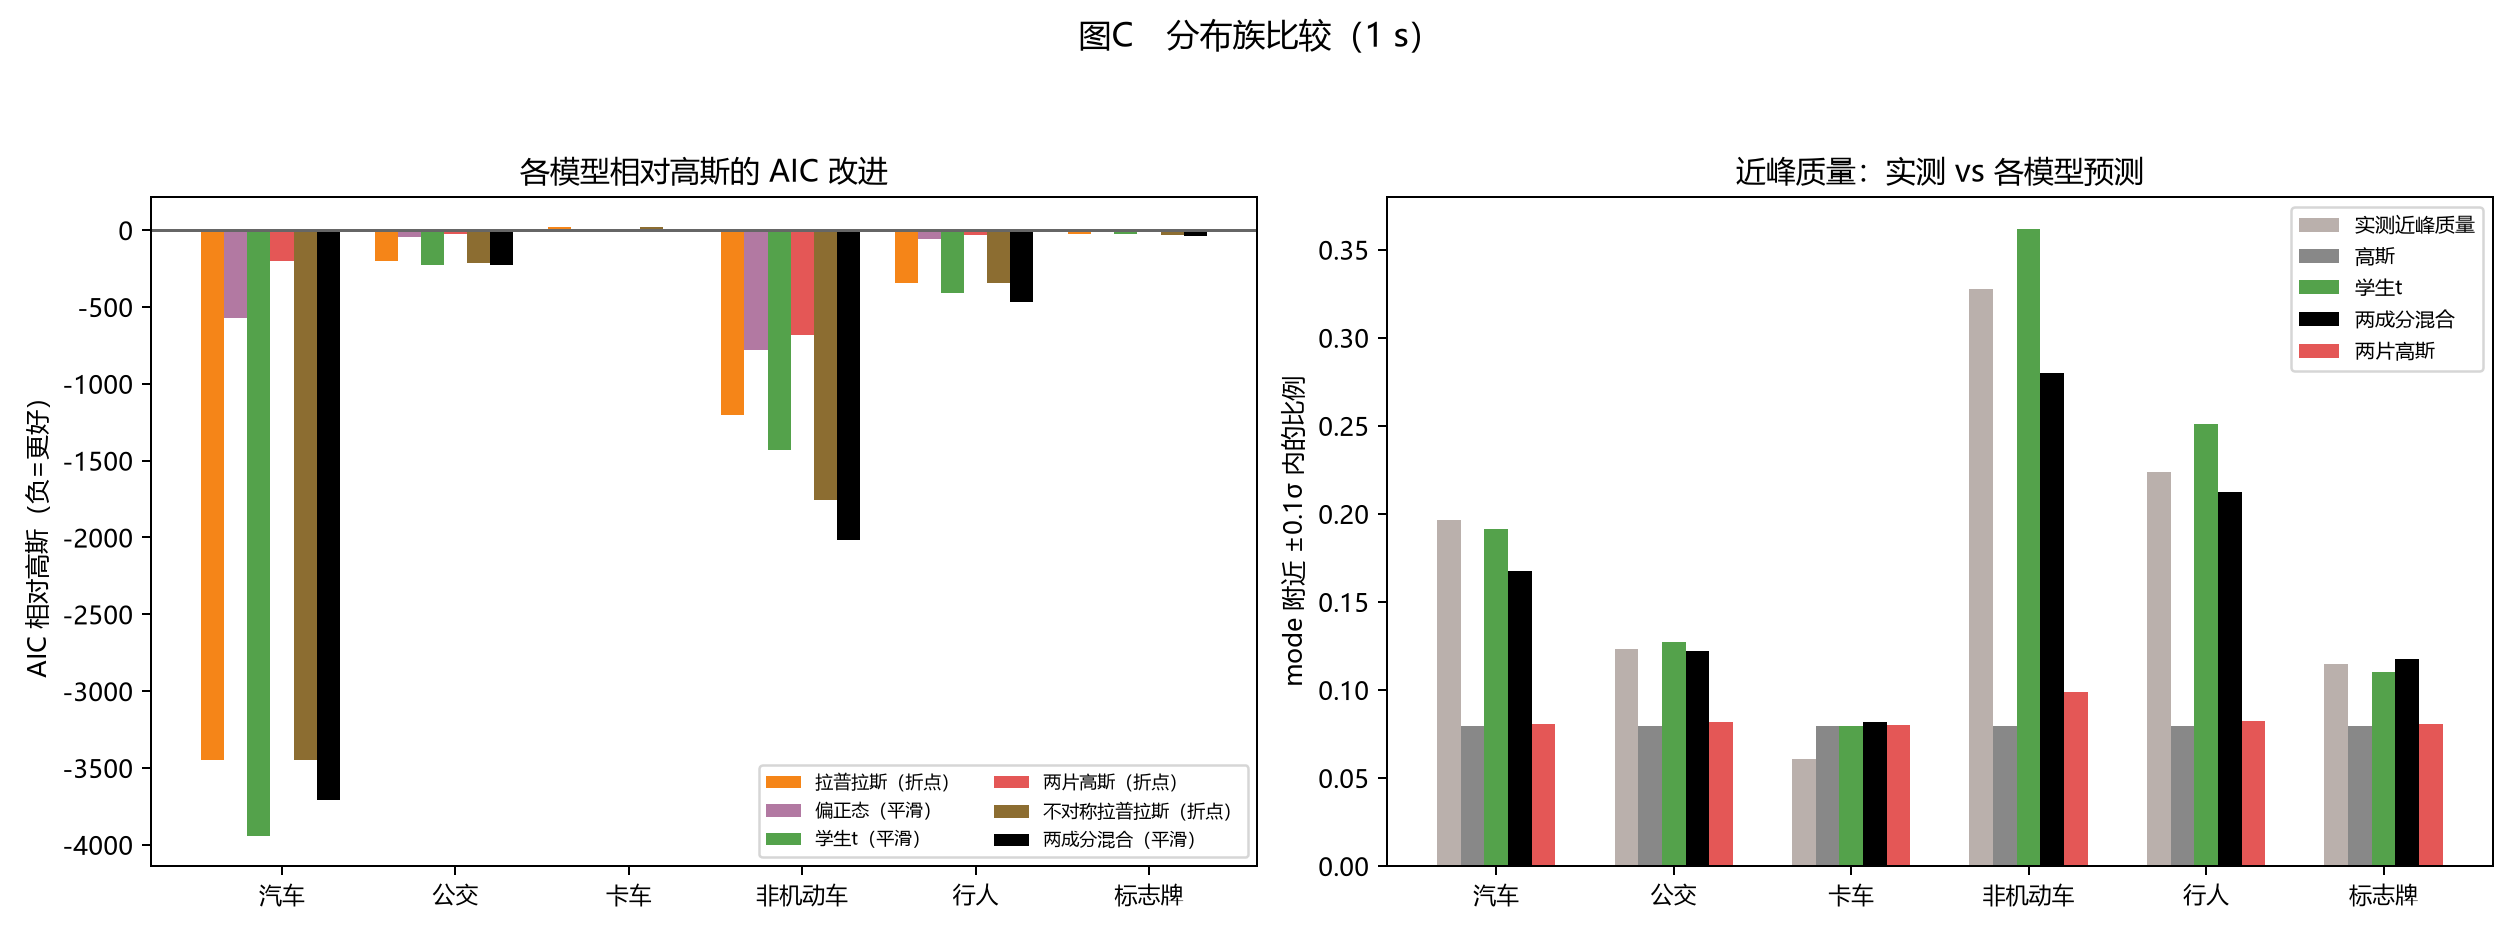
\includegraphics[width=0.92\linewidth]{fig_model_family_comparison.png}
\caption{分布族横评：各模型相对高斯的 AIC 改进与近峰质量对比。}
\end{figure}

\begin{figure}[h]\centering
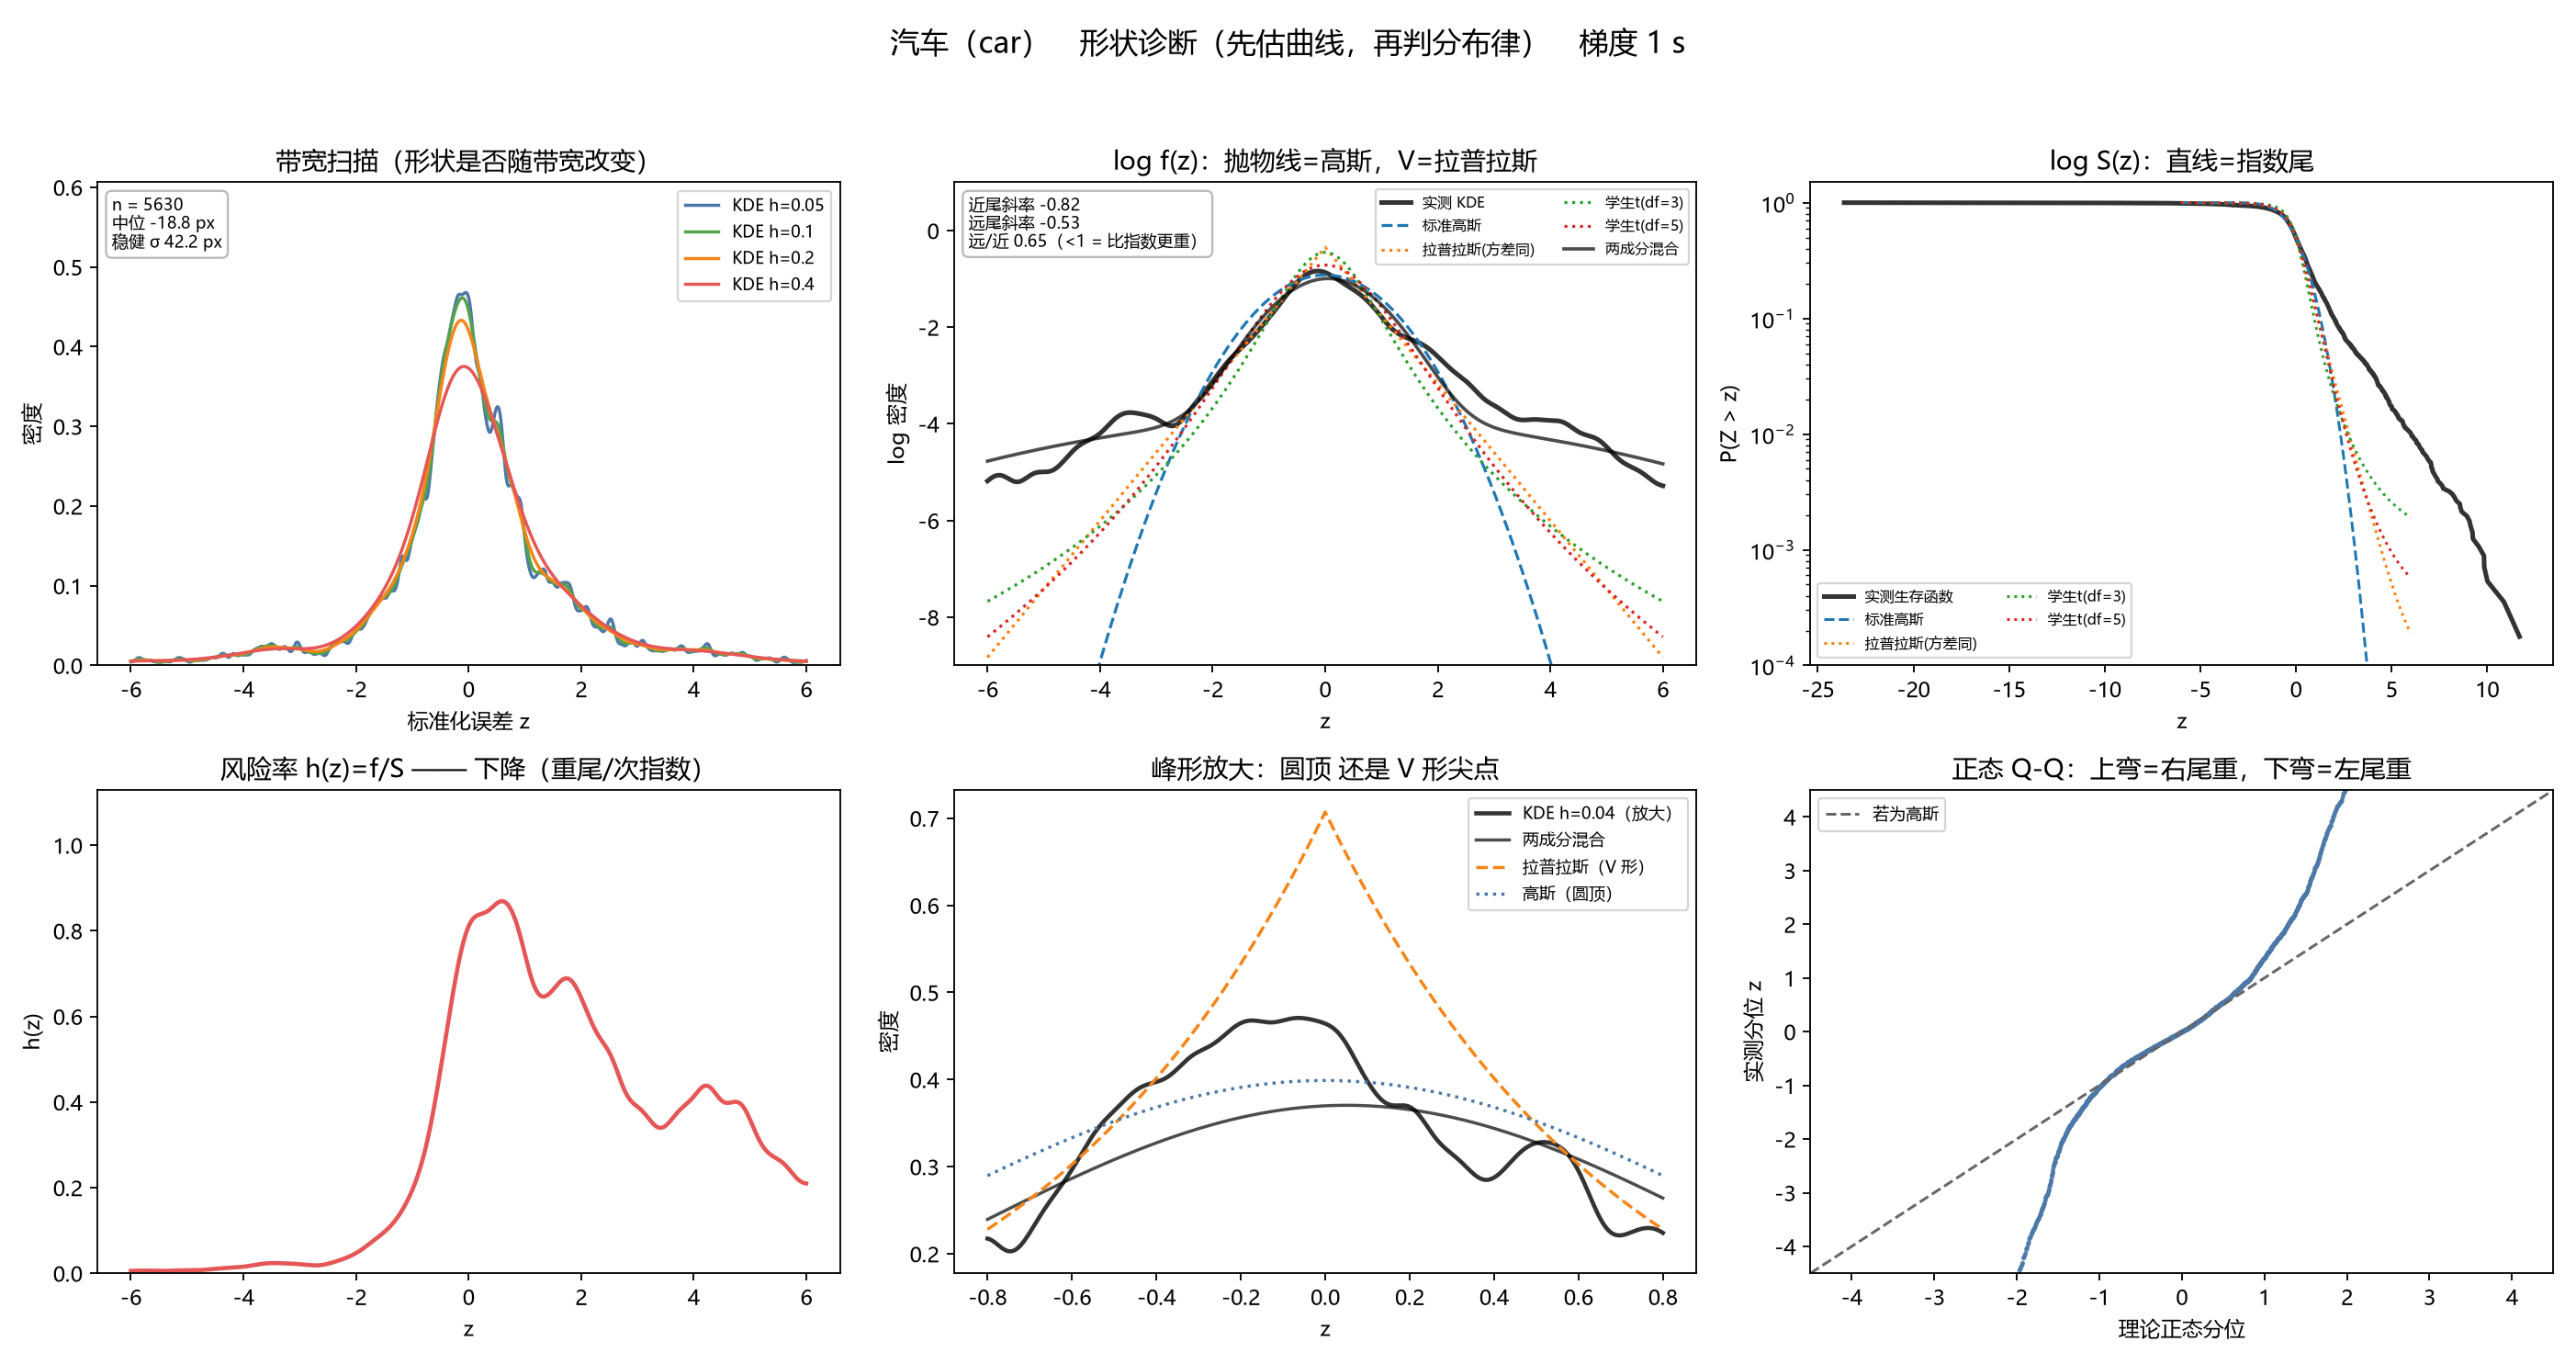
\includegraphics[width=0.92\linewidth]{fig_shape_car.png}
\caption{汽车类别的形状诊断六面板：带宽扫描、对数密度、生存函数、风险率、
峰形放大与正态分位图。}
\end{figure}

\end{document}
